%%%%%%%%%%%%%%%%%%%%%%%%%%%%%%%%%%%%%%%%%%%%%%%%%%%%%%%%%%%%%%%%%%%%%%%%

%%% LaTeX Template for AAMAS-2025 (based on sample-sigconf.tex)
%%% Prepared by the AAMAS-2025 Program Chairs based on the version from AAMAS-2025. 

%%%%%%%%%%%%%%%%%%%%%%%%%%%%%%%%%%%%%%%%%%%%%%%%%%%%%%%%%%%%%%%%%%%%%%%%

%%% Start your document with the \documentclass command.


%%% == IMPORTANT ==
%%% Use the first variant below for the final paper (including author information).
%%% Use the second variant below to anonymize your submission (no author information shown).
%%% For further information on anonymity and double-blind reviewing, 
%%% please consult the call for paper information
%%% https://aamas2025.org/index.php/conference/calls/submission-instructions-main-technical-track/

%%%% For anonymized submission, use this
\documentclass[sigconf,anonymous]{aamas} 

%%%% For camera-ready, use this
%\documentclass[sigconf]{aamas}

\usepackage{listings}
% \usepackage{xcolor}

\definecolor{codegreen}{rgb}{0,0.6,0}
\definecolor{codegray}{rgb}{0.5,0.5,0.5}
\definecolor{codepurple}{rgb}{0.58,0,82}
\definecolor{backcolour}{rgb}{0.95,0.95,0.92}
 
\lstdefinestyle{mystyle}{
    backgroundcolor=\color{backcolour},   
    commentstyle=\color{codegreen},
    keywordstyle=\color{magenta},
    numberstyle=\tiny\color{codegray},
    stringstyle=\color{codepurple},
    basicstyle=\footnotesize,
    breakatwhitespace=false,         
    breaklines=true,                 
    captionpos=b,                    
    keepspaces=true,                 
    numbers=left,                    
    numbersep=5pt,                  
    showspaces=false,                
    showstringspaces=false,
    showtabs=false,                  
    tabsize=2
}
 
\lstset{style=mystyle}

% --- Tickz
\usepackage{physics}
\usepackage{tikz}
\usepackage{amsmath}
\usepackage{mathdots}
% \usepackage{yhmath}
\usepackage{cancel}
\usepackage{color}
\usepackage{siunitx}
\usepackage{array}
\usepackage{cuted}
\usepackage{multirow}
% \usepackage{amssymb}
\usepackage{gensymb}
\usepackage{tabularx}
\usepackage{extarrows}
\usepackage{booktabs}
\usetikzlibrary{fadings}
\usetikzlibrary{patterns}
\usetikzlibrary{shadows.blur}
\usetikzlibrary{shapes}

% ---------

\usepackage{balance} % for balancing columns on the final page
\usepackage{csquotes}
% \usepackage{cite}
\newcommand{\probP}{I\kern-0.15em P}
\usepackage{etoolbox}
\patchcmd{\thebibliography}{\section*{\refname}}{}{}{}
% \usepackage{amsthm,amssymb,amsfonts}

\usepackage[T1]{fontenc}
\usepackage{graphicx}
\usepackage{hyperref}
\usepackage{color}
% \renewcommand\UrlFont{\color{blue}\rmfamily}

\usepackage[inline, shortlabels]{enumitem}
\usepackage{tabularx}
\usepackage{caption}
\usepackage{listings}
\usepackage{titlesec}
\usepackage{ragged2e}
% \usepackage[hyphens]{url}
\usepackage[linesnumbered,ruled,vlined]{algorithm2e}
\usepackage{float}

\usepackage[english]{babel}
\addto\extrasenglish{  
    \def\figureautorefname{Figure}
    \def\tableautorefname{Table}
    \def\algorithmautorefname{Algorithm}
    \def\sectionautorefname{Section}
    \def\subsectionautorefname{Subsection}
    \def\proofoutlineautorefname{Proof Outline}
}

\DeclareMathAlphabet\mathbfcal{OMS}{cmsy}{b}{n}

\newcommand{\supertiny}{\fontsize{1}{2}\selectfont}


%%%%%%%%%%%%%%%%%%%%%%%%%%%%%%%%%%%%%%%%%%%%%%%%%%%%%%%%%%%%%%%%%%%%%%%%

%%% AAMAS-2025 copyright block (do not change!)

\setcopyright{ifaamas}
\acmConference[AAMAS '25]{Proc.\@ of the 24th International Conference
on Autonomous Agents and Multiagent Systems (AAMAS 2025)}{May 19 -- 23, 2025}
{Detroit, Michigan, USA}{A.~El~Fallah~Seghrouchni, Y.~Vorobeychik, S.~Das, A.~Nowe (eds.)}
\copyrightyear{2025}
\acmYear{2025}
\acmDOI{}
\acmPrice{}
\acmISBN{}


%%%%%%%%%%%%%%%%%%%%%%%%%%%%%%%%%%%%%%%%%%%%%%%%%%%%%%%%%%%%%%%%%%%%%%%%

%%% == IMPORTANT ==
%%% Use this command to specify your EasyChair submission number.
%%% In anonymous mode, it will be printed on the first page.

\acmSubmissionID{<<EasyChair submission id>>}

%%% Use this command to specify the title of your paper.

\title[AAMAS-2025 CybMASDE]{A Method for Assisting Multi-Agent System Design Using Reinforcement Learning}

%%% Provide names, affiliations, and email addresses for all authors.

\author{Julien Soulé}
\affiliation{
  \institution{Univ. Grenoble Alpes}
  \city{Valence}
  \country{France}}
\email{julien.soule@lcis.grenoble-inp.fr}

\author{Jean-Paul Jamont}
\affiliation{
  \institution{Univ. Grenoble Alpes}
  \city{Valence}
  \country{France}}
\email{jean-paul.jamont@lcis.grenoble-inp.fr}

\author{Michel Occello}
\affiliation{
  \institution{Univ. Grenoble Alpes}
  \city{Valence}
  \country{France}}
\email{michel.occello@lcis.grenoble-inp.fr}

\author{Louis-Marie Traonouez}
\affiliation{
  \institution{Thales Land and Air Systems, BU IAS}
  \city{Rennes}
  \country{France}}
\email{louis-marie.traonouez@thalesgroup.com}

\author{Paul Théron}
\affiliation{
  \institution{AICA IWG}
  \city{La Guillermie}
  \country{France}}
\email{paul.theron@orange.fr}

\begin{abstract}
    Agent-Oriented Software Engineering (AOSE) methods typically rely on the designer's expertise to guide the development of a multi-agent system (MAS) that meets specific objectives within a given environment. Recent advancements in Multi-Agent Reinforcement Learning (MARL) suggest a more automated approach to exploring the design space. We introduce the SAMMASD (Semi-Automated MARL-based MAS Design) method, which integrates organizational specifications into MARL for MAS design and deployment. This method consists of four phases. The first phase models the real-world environment, objectives, and additional constraints—such as operational requirements—into a simulation. The second phase leverages multiple MARL algorithms to learn stable policies that achieve these objectives within the defined constraints. The third phase conducts a behavior analysis to infer emergent roles and objectives and to generate detailed "blueprints" for implementation. Finally, the development phase enables the automatic deployment of these policies in real-world environments, following validation in an emulated setting. We demonstrate SAMMASD in a warehouse flow management scenario involving robot agents, illustrating how the method can produce efficient and reliable MAS designs that streamline the design process.
\end{abstract}



%%% The code below was generated by the tool at http://dl.acm.org/ccs.cfm.
%%% Please replace this example with code appropriate for your own paper.


%%% Use this command to specify a few keywords describing your work.
%%% Keywords should be separated by commas.

\keywords{Agent-Oriented Software Engineering \and Multi-Agent Reinforcement Learning \and Assisted-Design \and Organizational Models}

%%%%%%%%%%%%%%%%%%%%%%%%%%%%%%%%%%%%%%%%%%%%%%%%%%%%%%%%%%%%%%%%%%%%%%%%

%%% Include any author-defined commands here.
         
% \newcommand{\BibTeX}{\rm B\kern-.05em{\sc i\kern-.025em b}\kern-.08em\TeX}

%%%%%%%%%%%%%%%%%%%%%%%%%%%%%%%%%%%%%%%%%%%%%%%%%%%%%%%%%%%%%%%%%%%%%%%%

\begin{document}

%%% The following commands remove the headers in your paper. For final 
%%% papers, these will be inserted during the pagination process.

\pagestyle{fancy}
\fancyhead{}

%%% The next command prints the information defined in the preamble.

\maketitle

%%%%%%%%%%%%%%%%%%%%%%%%%%%%%%%%%%%%%%%%%%%%%%%%%%%%%%%%%%%%%%%%%%%%%%%%

\section{Introduction}

Designing multi-agent systems (MAS) that can operate autonomously and efficiently in complex and dynamic environments is a significant challenge within the field of Agent-Oriented Software Engineering (AOSE). MAS are widely used across various applications, such as warehouse management, cybersecurity, and other domains where multiple agents must collaborate to achieve shared objectives. A crucial aspect of MAS design is ensuring that agent behaviors align with organizational requirements, including safety, explainability, and adaptability, while also allowing for efficient and robust operation in uncertain environments.

Traditional AOSE methodologies often rely heavily on expert knowledge to define organizational structures and guide agent behaviors, which can limit their scalability and adaptability to changing environments. Furthermore, while Multi-Agent Reinforcement Learning (MARL) has shown promise for automating aspects of MAS design, it frequently lacks mechanisms for incorporating explicit organizational constraints, which are essential for ensuring that agent behaviors remain interpretable and safe.

To address these limitations, we introduce a novel method, the \textbf{SAMMASD} (Semi-Automated MARL-based MAS Design) method, which integrates organizational specifications into MARL for the automated design and deployment of MAS. SAMMASD leverages the \textbf{MOISE+MARL} framework, which combines the organizational modeling capabilities of $\mathcal{M}OISE^+$ with the learning power of MARL. This integration allows for the enforcement of organizational constraints throughout the learning process, leading to the development of policies that are both effective and compliant with specified roles and objectives.

SAMMASD consists of four main phases:
\begin{enumerate*}[label=\roman*,itemjoin={; \quad}]
  \item modeling the target environment, objectives, and organizational constraints to create a simulation that faithfully reflects the system's dynamics
  \item training agent policies using a variety of MARL algorithms to optimize for defined objectives
  \item analyzing agent behaviors to infer roles, missions, and organizational structures, ensuring compliance with the \textbf{MOISE+MARL} specifications
  \item deploying the MAS into real-world environments, with steps for ensuring safety and adaptability.
\end{enumerate*}

In this paper, we apply the SAMMASD method within a simulated warehouse flow management scenario, utilizing the \textbf{CybMASDE} (Cyber Multi-Agent System Development Environment) tool to facilitate each phase. We evaluate the method's effectiveness based on output compliance, ease of use, automation, verification, and adaptability. Our findings demonstrate that SAMMASD offers a comprehensive approach to MAS design that bridges the gap between traditional AOSE methods and the emerging capabilities of MARL, while providing pathways for further refinement in real-time adaptability and deployment automation.

The remainder of this paper is organized as follows: \autoref{sec:related_works} presents related works in AOSE and MARL methodologies. \autoref{sec:sammasd_presentation} details the SAMMASD method and the MOISE+MARL framework. \autoref{sec:evaluation} discusses the experimental results from the warehouse management scenario. Finally, \autoref{sec:conclusion} concludes with insights on the contributions of SAMMASD and directions for future work.


\section{Related Works}
\label{sec:related_works}

This section presents a detailed analysis of Agent-Oriented Software Engineering (AOSE) methods for the design, development, and deployment of Multi-Agent Systems (MAS).

\begin{table*}[h!]
  \centering
  
  \footnotesize
  
  \caption{Comparison of AOSE methods according to key criteria for MAS design and deployment}
  \begin{tabular}{lcccccccccc}
  \textbf{Method} & \textbf{Automation} & \textbf{Adaptability} & \textbf{Accuracy} & \textbf{Safety} & \textbf{Performance} & \textbf{Explainability} & \textbf{Control} & \textbf{Scalability} & \textbf{Resilience} & \textbf{Modularity} \\
  \hline
  GAIA & Moderate & Moderate & Moderate & Low & High & Moderate & Moderate & Low & Low & Low \\
  TROPOS & Low & High & High & Moderate & High & Moderate & High & Moderate & Low & Low \\
  MaSE & Moderate & Moderate & High & High & High & High & High & Moderate & Low & Low \\
  Prometheus & High & Moderate & High & Moderate & High & Moderate & Moderate & Moderate & Low & Low \\
  O-MaSE & Moderate & High & High & High & Moderate & Moderate & High & Moderate & Moderate & Low \\
  INGENIAS & High & Moderate & High & Moderate & Moderate & Moderate & Moderate & Moderate & Low & Low \\
  ADELFE & Moderate & High & Moderate & Low & High & Low & Moderate & High & High & High \\
  KB-ORG & High & High & High & High & High & Moderate & High & High & Moderate & Low \\
  ASPECS & Moderate & High & High & High & High & Moderate & High & High & High & High \\
  TDF & Moderate & High & Moderate & Low & Moderate & High & High & Moderate & Moderate & Moderate \\
  ASPOI & High & High & Moderate & Moderate & Moderate & Low & High & High & High & Moderate \\
  \end{tabular}
  \label{tab:extended-aose-comparison}
  \end{table*}
  

\paragraph{GAIA}
The GAIA methodology \cite{wooldridge1999method} is one of the earliest frameworks that provided a structured approach for analyzing and designing MAS. GAIA supports moderate automation in design by defining agent roles, interactions, and responsibilities, though deployment relies heavily on manual adjustments. It shows moderate adaptability as roles and interactions can be updated, but scalability is limited for systems with a large number of agents. GAIA provides good accuracy by defining detailed roles and responsibilities, ensuring that agent actions align with the system's objectives. However, its safety features are minimal, and it requires extensive user input to implement safety constraints. GAIA's explainability is moderate since role and interaction definitions clarify agent behavior, but the overall resilience and modularity are low, as the methodology does not facilitate easy updates or independent component modifications.

\paragraph{TROPOS}
TROPOS \cite{bresciani2004tropos} is a goal-oriented AOSE methodology that integrates requirements analysis deeply into MAS development, which enhances adaptability by allowing agent goals to be modified as objectives change. TROPOS provides high accuracy due to its rigorous goal modeling process but suffers from low automation in the deployment phase. Its safety features are moderate, supporting early risk analysis, yet lacking runtime safety mechanisms. The performance is high as TROPOS ensures agents achieve well-defined goals, while its explainability benefits from the hierarchical goal structure. Control over agent behavior is high, as goals provide a clear structure, though scalability can be an issue as the number of goals and agents increases. TROPOS's resilience is limited since it lacks dynamic reconfiguration, and its modularity is low due to tightly coupled roles and objectives.

\paragraph{MaSE}
MaSE \cite{de1999multi} adopts a stepwise approach, from goal identification to deployment, which ensures high accuracy and moderate automation. It also offers moderate adaptability, as goal adjustments require revisiting design stages. MaSE excels in safety by embedding constraints directly into the agent behavior logic, providing users with high control over agent actions. It has moderate scalability, but the explainability is high since each step from analysis to design is well documented. MaSE, however, lacks resilience due to its static design structure, which limits flexibility in the face of environmental changes. Modularity is moderate as MaSE focuses on well-defined roles, although changing one component often impacts others.

\paragraph{Prometheus}
Prometheus \cite{padgham2005prometheus} emphasizes practical support for MAS design through tools that facilitate automation, especially in the design phase. It is highly adaptable, allowing for role adjustments to accommodate new objectives, and ensures high accuracy by clearly specifying roles and interactions. While safety mechanisms are provided during specification, runtime safety is not fully addressed. Prometheus excels in performance and control, as it tightly integrates design with implementation. Its explainability is moderate due to detailed documentation, though scalability can be challenging as systems grow. Resilience and modularity are limited by the framework's rigid structure, which complicates updates or modifications to isolated components.

\paragraph{O-MaSE}
O-MaSE \cite{garcia2007engineering} extends MaSE by introducing organizational structures, enhancing adaptability through its support for role dynamics. Automation is moderate, as organizational templates streamline some aspects of design, although deployment remains manual. O-MaSE achieves high accuracy by specifying organizational roles and objectives, and it provides strong safety features through organizational constraints. Performance is moderate, with agents achieving objectives under defined organizational rules, and explainability is enhanced by visualizing organizational structures. Control is high due to explicit role specifications, and scalability is better than MaSE due to the organizational focus. However, resilience and modularity are limited by the need to modify entire structures when changes are required.

\paragraph{INGENIAS}
INGENIAS \cite{gomez2003ingenias} offers comprehensive modeling support, enabling high automation and adaptability through its toolset, which facilitates design adjustments based on evolving requirements. It provides high accuracy due to detailed modeling but lacks strong safety features during runtime. Performance is moderate as the models ensure agent roles align with system goals. Explainability is limited, as INGENIAS can be complex and challenging to interpret, although control is high due to extensive specification options. Scalability is moderate, as the tool supports complex systems, but resilience and modularity are low, as INGENIAS models are highly integrated and difficult to modify independently.

\paragraph{ADELFE}
ADELFE \cite{gleize2008adelfe} focuses on Adaptive Multi-Agent Systems (AMAS), promoting adaptability through emergent behavior and self-organization. The methodology provides moderate automation with some tool support but requires manual adjustments in deployment. Accuracy is moderate, as agents adapt to environmental changes, but safety is low due to the unpredictable nature of emergent behaviors. ADELFE's performance and scalability are high, given the AMAS's ability to self-organize, though explainability can be low as emergent behaviors are difficult to interpret. Control is moderate as user input is limited to setting initial parameters, while resilience and modularity are strong due to the flexible and decentralized structure of AMAS.

\paragraph{KB-ORG}
KB-ORG \cite{corkill2008automated} leverages knowledge-based design to enable high automation, particularly in organizing and assigning roles based on environmental conditions. It is highly adaptable and accurate due to its knowledgeable pruning process, which ensures agent roles align with objectives while minimizing exploration effort. Safety is high as KB-ORG integrates safety requirements within organizational constraints, and it performs well even in large-scale environments. Explainability is moderate, given the complexity of knowledge-based decision-making, but control over agent behavior is high. Scalability is strong, though resilience may vary depending on the robustness of the knowledge base. Modularity is limited, as coordination roles are predefined and less flexible.

\paragraph{ASPECS}
ASPECS \cite{bernon2011aspecs} combines agent-oriented and holonic approaches to support complex hierarchical MAS. It offers moderate automation, with some tool support, and high adaptability and scalability due to the holonic architecture. ASPECS provides strong accuracy and safety by detailing roles and goals at multiple levels, but its explainability is moderate, as the multi-level structure can be challenging to comprehend. Control is high as holons allow for encapsulated role specifications, while resilience is supported by adaptive hierarchies that respond to environmental changes. Modularity is also high, as different levels can be modified independently.

\paragraph{TDF}
The Tactics Development Framework (TDF) \cite{winikoff2021tdf} introduces agile principles into AOSE, enhancing adaptability and explainability by aligning system requirements with agent actions through “User and System Stories.” Automation and scalability are moderate, while accuracy is high as agent actions are closely aligned with stakeholder requirements. Safety is low, but the method provides high control due to story-driven requirements. Resilience is moderate, as TDF adapts well to new requirements, and modularity is also moderate, allowing for changes to story definitions with minimal impact on the system.

\paragraph{ASPOI}
ASPOI \cite{isern2010organizational} enhances GAIA with support for complex organizational structures like hierarchies and coalitions, enabling high automation and adaptability. Its accuracy and control are high due to explicit organizational protocols, and it supports scalability by managing large MAS with organizational templates. Safety and resilience are moderate, as ASPOI allows for some dynamic reconfiguration, though its explainability can be low due to complex organization models. Modularity is also moderate, as ASPOI's organizational structures can be modified independently but require coordinated updates.

\paragraph{Synthesis and Comparison}
Table~\ref{tab:extended-aose-comparison} illustrates how current AOSE methodologies fare against key criteria. Most methods are limited in resilience and modularity, highlighting gaps in their ability to support dynamic changes and component independence. SAMMASD addresses these gaps by integrating the MOISE+MARL framework, which enforces robust control and adaptability. Its constraint guides enhance resilience and safety, while the multi-level organizational structure ensures modularity and scalability, making it a comprehensive solution for MAS design and deployment.



\section{Proposed Organizational Design Approach for MAS}
\label{sec:sammasd_presentation}

The core of the SAMMASD method is to consider the design of a MAS as a constrained optimization problem. The variable to be optimized is the \textbf{joint policy}, which represents the internal logic of the agents in determining their next actions. The goal is to maximize the cumulative reward under the given constraints. SAMMASD includes organizational specifications in MARL as additional constraints, allowing the user to control not only individual agent behaviors but also to manage the entire MAS through these specifications. We formalize this approach by proposing the MOISE+MARL framework and then using it to construct the four phases of our method.

\subsection{\textbf{MOISE+MARL Framework}}

The objective is to guide agent learning while adhering to organizational constraints in the form of roles and objectives, while ensuring sufficient efficiency of the learned policies within their environment. We formalize this concept by proposing the MOISE+MARL framework, which combines the formalism of a Decentralized Partially Observable Markov Decision Process (Dec-POMDP) with the $\mathcal{M}OISE^+$ organizational model.

\textbf{Dec-POMDP} \quad defined by a tuple $D = \langle N, S, A, P, R, \Omega, O, \gamma \rangle$, where:
%
\begin{itemize*}[label={},itemjoin={; }]
    \item $\mathcal{A}$ is the set of $N \in \mathbb{N}$ agents
    \item $S$, the set of possible states of the environment (including agents)
    \item $A = \times_{i=1}^N A_i $, the set of possible actions for each agent $i$
    \item $T: S \times A^N \to S$, the state transition function defining the next state $s'$ given a state $s$ under joint action $a$
    \item $R: S \times A^N \times  S \to \mathbb{R}$, the reward function assigning a reward $r$ to each transition $(s, a, s')$
    \item $\Omega = \times_{i=1}^N \Omega_i $ is the set of possible observations for each agent $i$
    \item $O: S \times A \to \Omega$ is the observation function defining the next observation $\omega$ of an agent when taking action $a$ in state $s$
    \item $\gamma \in [0, 1] $ is the discount factor.
\end{itemize*}

$\mathbf{\mathcal{M}OISE^+}$ \quad defined by a tuple $\mathcal{OS} = \langle \mathcal{SS}, \mathcal{FS}, \mathcal{DS} \rangle$. Here, we present a minimal version of the $\mathcal{M}OISE^+$ formalism:
\begin{itemize*}[label={},itemjoin={; }]
    \item $\mathcal{SS} = \langle \mathcal{R} \rangle$, structural specifications defined by a set of roles $\mathcal{R}$
    \item $\mathcal{FS} = \langle \mathcal{G}, \mathcal{M}, mo \rangle$, functional specifications are a set of objectives $\mathcal{G}$, a set of missions $\mathcal{M}$, and a function $mo: \mathcal{M} \to \mathcal{P}(\mathcal{G} \times [0,1])$ associating a mission $m \in \mathcal{M}$ with a set of objectives, each weighted by a value $\{(g_1,w_0), (g_2,w_1)\dots\}, w_i \in [0,1], g_i \in \mathcal{G}$
    \item $\mathcal{DS} = \mathcal{R} \times \mathcal{M} \times T_c \times \{0,1\}$, deontic specifications as a set of quadruples $(\rho_a, m, \allowbreak t_c, p)$, meaning that an agent playing the role $\rho_a \in \mathcal{R}$ is permitted (if $p = 0$) or obligated (if $p = 1$) to engage in mission $m \in \mathcal{M}, \ m \subseteq \mathcal{G}$ for a given time constraint $t_c \in \mathcal{TC}, t_c = \mathcal{P}(N)$ specifying a period during which permission/obligation is valid.
\end{itemize*}

The \textbf{Constraint Guides} \quad are three new relations introduced to describe the logic of the roles and objectives of $\mathcal{M}OISE^+$ in the Dec-POMDP formalism:

\begin{itemize}
    \item \textbf{Role Action Guide} (RAG) \quad $rag: H \times \Omega \rightarrow \mathcal{P}(A \times \mathbb{R})$, the relation that models a role as a set of rules which, for each pair consisting of a history $h \in H$ and an observation received by the agent $\omega \in \Omega$, associates expected actions $A \in \mathcal{P}(A)$ each associated with a constraint hardness $ch \in [0,1]$ ($ch = 1$ by default). By restricting the choice of the next action among those authorized, the agent is forced to adhere to the expected behavior of the role.
    \item \textbf{Role Reward Guide} (RRG) \quad $rrg: H \times \Omega \times A \to \mathbb{R} = \{r_m \text{ if } a \notin A_\omega \text{, } rag(h, \omega) = A_\omega \times \mathbb{R} \text{, } h \in H; \text{ else } 0\}$, the relation that models a role by adding a penalty $r_m$ to the global reward if the last action chosen by the agent $a \in A$ is not authorized. This is intended to encourage the agent to adhere to the expected behavior of a role.
    \item \textbf{Goal Reward Guide} (GRG) \quad $grg: H \rightarrow \mathbb{R}$, the relation that models a goal as a soft constraint by adding a bonus $r_b \in \mathbb{R}$ to the global reward if the agent's history $h \in H$ contains a characteristic sub-sequence $h_g \in H_g$ of the goal, encouraging the agent to find a way to reach it.
\end{itemize}

\begin{figure*}[h!]
  \centering
  


\tikzset{every picture/.style={line width=0.75pt}} %set default line width to 0.75pt        

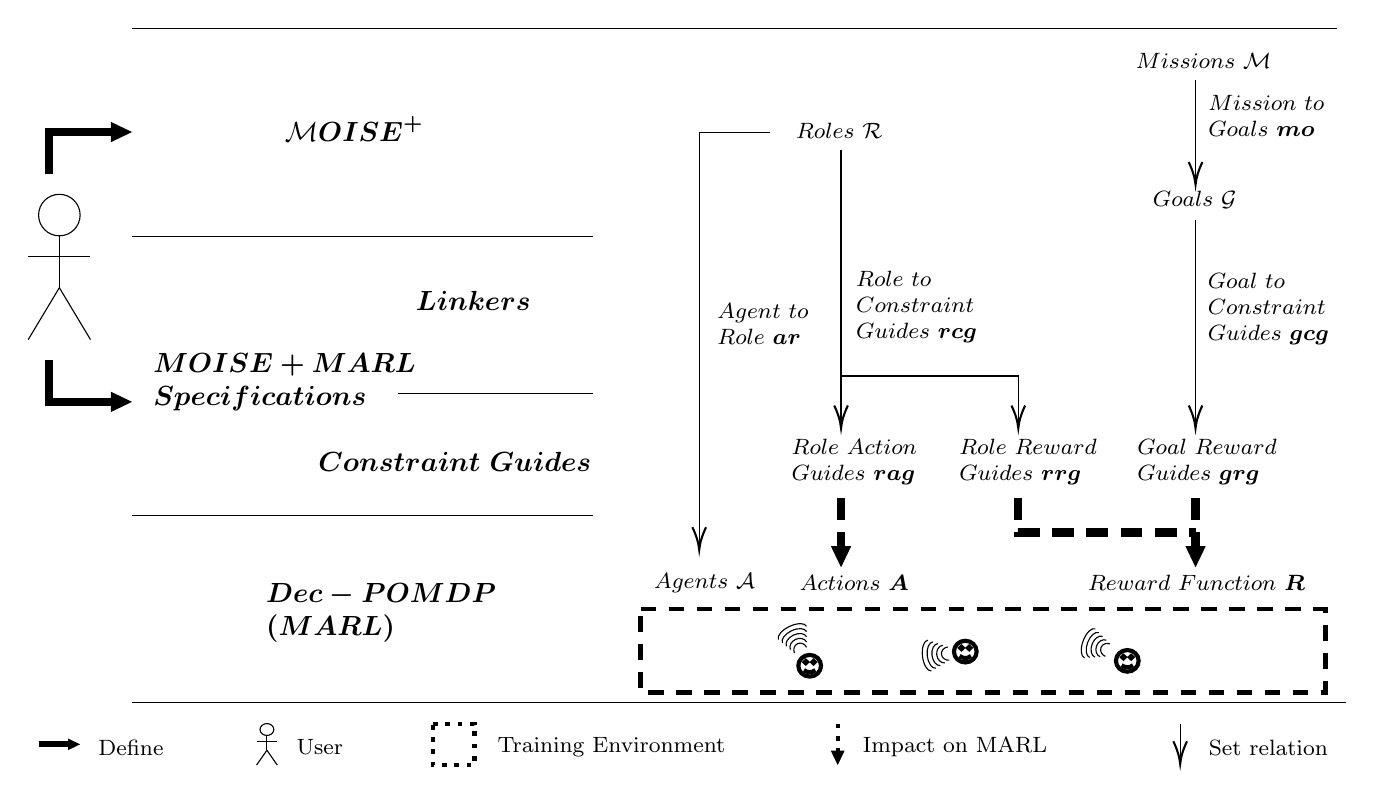
\begin{tikzpicture}[x=0.75pt,y=0.75pt,yscale=-1,xscale=1]
%uncomment if require: \path (0,2584); %set diagram left start at 0, and has height of 2584

%Straight Lines [id:da43492967264827187] 
\draw    (60,2000.54) -- (282.04,2000.54) ;
%Straight Lines [id:da5909021483617971] 
\draw    (572.41,1925.14) -- (572.41,1973.4) ;
\draw [shift={(572.41,1975.4)}, rotate = 270] [color={rgb, 255:red, 0; green, 0; blue, 0 }  ][line width=0.75]    (10.93,-3.29) .. controls (6.95,-1.4) and (3.31,-0.3) .. (0,0) .. controls (3.31,0.3) and (6.95,1.4) .. (10.93,3.29)   ;
%Straight Lines [id:da21005556631392852] 
\draw    (60,2134.58) -- (282.04,2134.58) ;
%Straight Lines [id:da3719427574917362] 
\draw    (188,2076) -- (282,2076) ;
%Straight Lines [id:da9250384002206431] 
\draw    (60,2225) -- (129,2225) -- (143,2225) -- (645,2225) ;
%Straight Lines [id:da8740103748997392] 
\draw    (60,1900.01) -- (640.73,1900.01) ;
%Straight Lines [id:da7641738582470461] 
\draw    (367.45,1950.27) -- (333.28,1950.27) -- (333.28,2149.33) ;
\draw [shift={(333.28,2151.33)}, rotate = 270] [color={rgb, 255:red, 0; green, 0; blue, 0 }  ][line width=0.75]    (10.93,-3.29) .. controls (6.95,-1.4) and (3.31,-0.3) .. (0,0) .. controls (3.31,0.3) and (6.95,1.4) .. (10.93,3.29)   ;
%Straight Lines [id:da17224242539642898] 
\draw    (401.61,1958.65) -- (401.61,2067.56) -- (401.61,2067.56) -- (401.61,2090.69) ;
\draw [shift={(401.61,2092.69)}, rotate = 270] [color={rgb, 255:red, 0; green, 0; blue, 0 }  ][line width=0.75]    (10.93,-3.29) .. controls (6.95,-1.4) and (3.31,-0.3) .. (0,0) .. controls (3.31,0.3) and (6.95,1.4) .. (10.93,3.29)   ;
%Straight Lines [id:da195049508631697] 
\draw    (401.61,2067.56) -- (487.01,2067.56) -- (487.01,2090.69) ;
\draw [shift={(487.01,2092.69)}, rotate = 270] [color={rgb, 255:red, 0; green, 0; blue, 0 }  ][line width=0.75]    (10.93,-3.29) .. controls (6.95,-1.4) and (3.31,-0.3) .. (0,0) .. controls (3.31,0.3) and (6.95,1.4) .. (10.93,3.29)   ;
%Straight Lines [id:da5129636072802843] 
\draw [line width=3]  [dash pattern={on 7.88pt off 4.5pt}]  (401.61,2126.2) -- (401.61,2153.71) ;
\draw [shift={(401.61,2159.71)}, rotate = 270] [fill={rgb, 255:red, 0; green, 0; blue, 0 }  ][line width=0.08]  [draw opacity=0] (10.18,-4.89) -- (0,0) -- (10.18,4.89) -- cycle    ;
%Straight Lines [id:da21235341061359447] 
\draw    (572.41,1992.16) -- (572.41,2090.69) ;
\draw [shift={(572.41,2092.69)}, rotate = 270] [color={rgb, 255:red, 0; green, 0; blue, 0 }  ][line width=0.75]    (10.93,-3.29) .. controls (6.95,-1.4) and (3.31,-0.3) .. (0,0) .. controls (3.31,0.3) and (6.95,1.4) .. (10.93,3.29)   ;
%Straight Lines [id:da8480030801651877] 
\draw [line width=3]  [dash pattern={on 7.88pt off 4.5pt}]  (572.41,2126.2) -- (572.41,2153.71) ;
\draw [shift={(572.41,2159.71)}, rotate = 270] [fill={rgb, 255:red, 0; green, 0; blue, 0 }  ][line width=0.08]  [draw opacity=0] (10.18,-4.89) -- (0,0) -- (10.18,4.89) -- cycle    ;
%Straight Lines [id:da489070602914107] 
\draw [line width=3]  [dash pattern={on 7.88pt off 4.5pt}]  (487.01,2126.2) -- (487.01,2142.95) -- (572.41,2142.95) ;
%Straight Lines [id:da28979276774504226] 
\draw [line width=1.5]  [dash pattern={on 1.69pt off 2.76pt}]  (400,2235) -- (400,2251) ;
\draw [shift={(400,2255)}, rotate = 270] [fill={rgb, 255:red, 0; green, 0; blue, 0 }  ][line width=0.08]  [draw opacity=0] (6.97,-3.35) -- (0,0) -- (6.97,3.35) -- cycle    ;
%Straight Lines [id:da09094883516825636] 
\draw    (565,2235) -- (565,2252.46) ;
\draw [shift={(565,2254.46)}, rotate = 270] [color={rgb, 255:red, 0; green, 0; blue, 0 }  ][line width=0.75]    (10.93,-3.29) .. controls (6.95,-1.4) and (3.31,-0.3) .. (0,0) .. controls (3.31,0.3) and (6.95,1.4) .. (10.93,3.29)   ;
%Shape: Arc [id:dp17514862021583588] 
\draw  [draw opacity=0] (371.45,2194.53) .. controls (370.65,2192.81) and (373.03,2189.98) .. (376.76,2188.21) .. controls (380.49,2186.44) and (384.17,2186.4) .. (384.97,2188.12) .. controls (384.97,2188.12) and (384.97,2188.12) .. (384.97,2188.12) -- (378.21,2191.32) -- cycle ; \draw   (371.45,2194.53) .. controls (370.65,2192.81) and (373.03,2189.98) .. (376.76,2188.21) .. controls (380.49,2186.44) and (384.17,2186.4) .. (384.97,2188.12) .. controls (384.97,2188.12) and (384.97,2188.12) .. (384.97,2188.12) ;  
%Shape: Arc [id:dp5560864173171258] 
\draw  [draw opacity=0] (373.39,2196.15) .. controls (373.39,2196.15) and (373.39,2196.15) .. (373.39,2196.15) .. controls (372.58,2194.43) and (374.53,2191.8) .. (377.73,2190.29) .. controls (380.93,2188.77) and (384.17,2188.93) .. (384.98,2190.65) -- (379.18,2193.4) -- cycle ; \draw   (373.39,2196.15) .. controls (373.39,2196.15) and (373.39,2196.15) .. (373.39,2196.15) .. controls (372.58,2194.43) and (374.53,2191.8) .. (377.73,2190.29) .. controls (380.93,2188.77) and (384.17,2188.93) .. (384.98,2190.65) ;  
%Shape: Arc [id:dp5165448368957106] 
\draw  [draw opacity=0] (375.32,2197.77) .. controls (375.32,2197.77) and (375.32,2197.77) .. (375.32,2197.77) .. controls (374.52,2196.05) and (376.03,2193.63) .. (378.7,2192.36) .. controls (381.36,2191.1) and (384.18,2191.47) .. (384.98,2193.19) -- (380.15,2195.48) -- cycle ; \draw   (375.32,2197.77) .. controls (375.32,2197.77) and (375.32,2197.77) .. (375.32,2197.77) .. controls (374.52,2196.05) and (376.03,2193.63) .. (378.7,2192.36) .. controls (381.36,2191.1) and (384.18,2191.47) .. (384.98,2193.19) ;  
%Shape: Arc [id:dp830154522734809] 
\draw  [draw opacity=0] (377.25,2199.39) .. controls (377.25,2199.39) and (377.25,2199.39) .. (377.25,2199.39) .. controls (376.45,2197.67) and (377.53,2195.45) .. (379.67,2194.44) .. controls (381.8,2193.43) and (384.18,2194) .. (384.98,2195.73) -- (381.12,2197.56) -- cycle ; \draw   (377.25,2199.39) .. controls (377.25,2199.39) and (377.25,2199.39) .. (377.25,2199.39) .. controls (376.45,2197.67) and (377.53,2195.45) .. (379.67,2194.44) .. controls (381.8,2193.43) and (384.18,2194) .. (384.98,2195.73) ;  
%Shape: Arc [id:dp3508601232471842] 
\draw  [draw opacity=0] (379.19,2201.01) .. controls (379.19,2201.01) and (379.19,2201.01) .. (379.19,2201.01) .. controls (378.39,2199.29) and (379.03,2197.28) .. (380.63,2196.52) .. controls (382.23,2195.76) and (384.18,2196.54) .. (384.98,2198.26) -- (382.09,2199.64) -- cycle ; \draw   (379.19,2201.01) .. controls (379.19,2201.01) and (379.19,2201.01) .. (379.19,2201.01) .. controls (378.39,2199.29) and (379.03,2197.28) .. (380.63,2196.52) .. controls (382.23,2195.76) and (384.18,2196.54) .. (384.98,2198.26) ;  

%Shape: Smiley Face [id:dp6280323748435761] 
\draw  [line width=1.5]  (381.03,2207.14) .. controls (381.03,2204.26) and (383.48,2201.92) .. (386.5,2201.92) .. controls (389.52,2201.92) and (391.97,2204.26) .. (391.97,2207.14) .. controls (391.97,2210.02) and (389.52,2212.36) .. (386.5,2212.36) .. controls (383.48,2212.36) and (381.03,2210.02) .. (381.03,2207.14) -- cycle ; \draw  [line width=1.5]  (384.1,2205.37) .. controls (384.1,2205.08) and (384.34,2204.85) .. (384.64,2204.85) .. controls (384.94,2204.85) and (385.19,2205.08) .. (385.19,2205.37) .. controls (385.19,2205.66) and (384.94,2205.89) .. (384.64,2205.89) .. controls (384.34,2205.89) and (384.1,2205.66) .. (384.1,2205.37) -- cycle ; \draw  [line width=1.5]  (387.81,2205.37) .. controls (387.81,2205.08) and (388.06,2204.85) .. (388.36,2204.85) .. controls (388.66,2204.85) and (388.91,2205.08) .. (388.91,2205.37) .. controls (388.91,2205.66) and (388.66,2205.89) .. (388.36,2205.89) .. controls (388.06,2205.89) and (387.81,2205.66) .. (387.81,2205.37) -- cycle ; \draw  [line width=1.5]  (383.77,2209.23) .. controls (385.59,2210.62) and (387.41,2210.62) .. (389.24,2209.23) ;

%Shape: Rectangle [id:dp8134535680778092] 
\draw  [dash pattern={on 5.63pt off 4.5pt}][line width=1.5]  (305,2180) -- (635,2180) -- (635,2220) -- (305,2220) -- cycle ;
%Shape: Smiley Face [id:dp004477643727426317] 
\draw  [line width=1.5]  (534.06,2204.78) .. controls (534.06,2201.9) and (536.51,2199.57) .. (539.53,2199.57) .. controls (542.55,2199.57) and (545,2201.9) .. (545,2204.78) .. controls (545,2207.66) and (542.55,2210) .. (539.53,2210) .. controls (536.51,2210) and (534.06,2207.66) .. (534.06,2204.78) -- cycle ; \draw  [line width=1.5]  (537.13,2203.01) .. controls (537.13,2202.72) and (537.37,2202.49) .. (537.67,2202.49) .. controls (537.97,2202.49) and (538.22,2202.72) .. (538.22,2203.01) .. controls (538.22,2203.3) and (537.97,2203.53) .. (537.67,2203.53) .. controls (537.37,2203.53) and (537.13,2203.3) .. (537.13,2203.01) -- cycle ; \draw  [line width=1.5]  (540.84,2203.01) .. controls (540.84,2202.72) and (541.09,2202.49) .. (541.39,2202.49) .. controls (541.69,2202.49) and (541.94,2202.72) .. (541.94,2203.01) .. controls (541.94,2203.3) and (541.69,2203.53) .. (541.39,2203.53) .. controls (541.09,2203.53) and (540.84,2203.3) .. (540.84,2203.01) -- cycle ; \draw  [line width=1.5]  (536.8,2206.87) .. controls (538.62,2208.26) and (540.44,2208.26) .. (542.27,2206.87) ;
%Shape: Arc [id:dp5812366585646123] 
\draw  [draw opacity=0] (518.89,2203.35) .. controls (518.89,2203.35) and (518.89,2203.35) .. (518.89,2203.35) .. controls (517.11,2202.67) and (516.83,2198.99) .. (518.27,2195.13) .. controls (519.7,2191.26) and (522.31,2188.67) .. (524.09,2189.35) -- (521.49,2196.35) -- cycle ; \draw   (518.89,2203.35) .. controls (518.89,2203.35) and (518.89,2203.35) .. (518.89,2203.35) .. controls (517.11,2202.67) and (516.83,2198.99) .. (518.27,2195.13) .. controls (519.7,2191.26) and (522.31,2188.67) .. (524.09,2189.35) ;  
%Shape: Arc [id:dp844447259400031] 
\draw  [draw opacity=0] (521.41,2203.16) .. controls (521.41,2203.16) and (521.41,2203.16) .. (521.41,2203.16) .. controls (519.63,2202.49) and (519.18,2199.25) .. (520.41,2195.94) .. controls (521.64,2192.63) and (524.08,2190.49) .. (525.86,2191.17) -- (523.64,2197.17) -- cycle ; \draw   (521.41,2203.16) .. controls (521.41,2203.16) and (521.41,2203.16) .. (521.41,2203.16) .. controls (519.63,2202.49) and (519.18,2199.25) .. (520.41,2195.94) .. controls (521.64,2192.63) and (524.08,2190.49) .. (525.86,2191.17) ;  
%Shape: Arc [id:dp10402158940144113] 
\draw  [draw opacity=0] (523.93,2202.98) .. controls (523.93,2202.98) and (523.93,2202.98) .. (523.93,2202.98) .. controls (522.15,2202.3) and (521.54,2199.52) .. (522.56,2196.76) .. controls (523.59,2194) and (525.86,2192.31) .. (527.64,2192.98) -- (525.78,2197.98) -- cycle ; \draw   (523.93,2202.98) .. controls (523.93,2202.98) and (523.93,2202.98) .. (523.93,2202.98) .. controls (522.15,2202.3) and (521.54,2199.52) .. (522.56,2196.76) .. controls (523.59,2194) and (525.86,2192.31) .. (527.64,2192.98) ;  
%Shape: Arc [id:dp1981700585306363] 
\draw  [draw opacity=0] (526.45,2202.8) .. controls (526.45,2202.8) and (526.45,2202.8) .. (526.45,2202.8) .. controls (526.45,2202.8) and (526.45,2202.8) .. (526.45,2202.8) .. controls (524.67,2202.12) and (523.89,2199.78) .. (524.71,2197.57) .. controls (525.53,2195.36) and (527.64,2194.12) .. (529.42,2194.8) -- (527.93,2198.8) -- cycle ; \draw   (526.45,2202.8) .. controls (526.45,2202.8) and (526.45,2202.8) .. (526.45,2202.8) .. controls (526.45,2202.8) and (526.45,2202.8) .. (526.45,2202.8) .. controls (524.67,2202.12) and (523.89,2199.78) .. (524.71,2197.57) .. controls (525.53,2195.36) and (527.64,2194.12) .. (529.42,2194.8) ;  
%Shape: Arc [id:dp4685733765037834] 
\draw  [draw opacity=0] (528.97,2202.61) .. controls (528.97,2202.61) and (528.97,2202.61) .. (528.97,2202.61) .. controls (527.19,2201.94) and (526.24,2200.04) .. (526.86,2198.39) .. controls (527.47,2196.73) and (529.42,2195.94) .. (531.19,2196.61) -- (530.08,2199.61) -- cycle ; \draw   (528.97,2202.61) .. controls (528.97,2202.61) and (528.97,2202.61) .. (528.97,2202.61) .. controls (527.19,2201.94) and (526.24,2200.04) .. (526.86,2198.39) .. controls (527.47,2196.73) and (529.42,2195.94) .. (531.19,2196.61) ;  


%Shape: Smiley Face [id:dp678720544610355] 
\draw  [line width=1.5]  (456.01,2200.32) .. controls (456.01,2197.44) and (458.46,2195.1) .. (461.48,2195.1) .. controls (464.5,2195.1) and (466.95,2197.44) .. (466.95,2200.32) .. controls (466.95,2203.2) and (464.5,2205.54) .. (461.48,2205.54) .. controls (458.46,2205.54) and (456.01,2203.2) .. (456.01,2200.32) -- cycle ; \draw  [line width=1.5]  (459.07,2198.55) .. controls (459.07,2198.26) and (459.32,2198.03) .. (459.62,2198.03) .. controls (459.92,2198.03) and (460.17,2198.26) .. (460.17,2198.55) .. controls (460.17,2198.84) and (459.92,2199.07) .. (459.62,2199.07) .. controls (459.32,2199.07) and (459.07,2198.84) .. (459.07,2198.55) -- cycle ; \draw  [line width=1.5]  (462.79,2198.55) .. controls (462.79,2198.26) and (463.04,2198.03) .. (463.34,2198.03) .. controls (463.64,2198.03) and (463.89,2198.26) .. (463.89,2198.55) .. controls (463.89,2198.84) and (463.64,2199.07) .. (463.34,2199.07) .. controls (463.04,2199.07) and (462.79,2198.84) .. (462.79,2198.55) -- cycle ; \draw  [line width=1.5]  (458.75,2202.41) .. controls (460.57,2203.8) and (462.39,2203.8) .. (464.21,2202.41) ;
%Shape: Arc [id:dp5571086156109115] 
\draw  [draw opacity=0] (445.12,2209.64) .. controls (445.12,2209.64) and (445.12,2209.64) .. (445.12,2209.64) .. controls (443.23,2209.84) and (441.31,2206.68) .. (440.85,2202.59) .. controls (440.38,2198.49) and (441.54,2195.01) .. (443.43,2194.81) -- (444.28,2202.23) -- cycle ; \draw   (445.12,2209.64) .. controls (445.12,2209.64) and (445.12,2209.64) .. (445.12,2209.64) .. controls (443.23,2209.84) and (441.31,2206.68) .. (440.85,2202.59) .. controls (440.38,2198.49) and (441.54,2195.01) .. (443.43,2194.81) ;  
%Shape: Arc [id:dp3637690398697262] 
\draw  [draw opacity=0] (447.29,2208.35) .. controls (445.39,2208.54) and (443.53,2205.86) .. (443.13,2202.35) .. controls (442.73,2198.84) and (443.94,2195.83) .. (445.84,2195.64) -- (446.56,2201.99) -- cycle ; \draw   (447.29,2208.35) .. controls (445.39,2208.54) and (443.53,2205.86) .. (443.13,2202.35) .. controls (442.73,2198.84) and (443.94,2195.83) .. (445.84,2195.64) ;  
%Shape: Arc [id:dp8671538897269329] 
\draw  [draw opacity=0] (449.45,2207.05) .. controls (447.56,2207.25) and (445.75,2205.03) .. (445.42,2202.11) .. controls (445.09,2199.18) and (446.35,2196.65) .. (448.25,2196.46) -- (448.85,2201.75) -- cycle ; \draw   (449.45,2207.05) .. controls (447.56,2207.25) and (445.75,2205.03) .. (445.42,2202.11) .. controls (445.09,2199.18) and (446.35,2196.65) .. (448.25,2196.46) ;  
%Shape: Arc [id:dp11882848969606119] 
\draw  [draw opacity=0] (451.62,2205.75) .. controls (449.72,2205.95) and (447.97,2204.21) .. (447.71,2201.87) .. controls (447.44,2199.53) and (448.76,2197.48) .. (450.65,2197.28) -- (451.14,2201.52) -- cycle ; \draw   (451.62,2205.75) .. controls (449.72,2205.95) and (447.97,2204.21) .. (447.71,2201.87) .. controls (447.44,2199.53) and (448.76,2197.48) .. (450.65,2197.28) ;  
%Shape: Arc [id:dp21458661066028384] 
\draw  [draw opacity=0] (453.78,2204.46) .. controls (451.89,2204.65) and (450.19,2203.39) .. (449.99,2201.63) .. controls (449.79,2199.88) and (451.17,2198.3) .. (453.06,2198.1) -- (453.42,2201.28) -- cycle ; \draw   (453.78,2204.46) .. controls (451.89,2204.65) and (450.19,2203.39) .. (449.99,2201.63) .. controls (449.79,2199.88) and (451.17,2198.3) .. (453.06,2198.1) ;  


%Shape: Rectangle [id:dp2900769639798859] 
\draw  [dash pattern={on 1.69pt off 2.76pt}][line width=1.5]  (205,2235) -- (225,2235) -- (225,2255) -- (205,2255) -- cycle ;
%Shape: Ellipse [id:dp12129322056737624] 
\draw   (15,1990) .. controls (15,1984.48) and (19.48,1980) .. (25,1980) .. controls (30.52,1980) and (35,1984.48) .. (35,1990) .. controls (35,1995.52) and (30.52,2000) .. (25,2000) .. controls (19.48,2000) and (15,1995.52) .. (15,1990) -- cycle ;
%Straight Lines [id:da3929164746972045] 
\draw    (25,2000) -- (25,2025) ;
%Straight Lines [id:da6768533991948997] 
\draw    (25,2025) -- (10,2050) ;
%Straight Lines [id:da8211797605779181] 
\draw    (25,2025) -- (40,2050) ;
%Straight Lines [id:da9570871044361624] 
\draw    (40,2010) -- (10,2010) ;

%Shape: Boxed Line [id:dp9135285972031537] 
\draw [line width=3]    (20,1970) -- (20,1950) -- (54,1950) ;
\draw [shift={(60,1950)}, rotate = 180] [fill={rgb, 255:red, 0; green, 0; blue, 0 }  ][line width=0.08]  [draw opacity=0] (10.18,-4.89) -- (0,0) -- (10.18,4.89) -- cycle    ;
%Shape: Boxed Line [id:dp5029508503979006] 
\draw [line width=3]    (20,2060) -- (20,2080) -- (54,2080) ;
\draw [shift={(60,2080)}, rotate = 180] [fill={rgb, 255:red, 0; green, 0; blue, 0 }  ][line width=0.08]  [draw opacity=0] (10.18,-4.89) -- (0,0) -- (10.18,4.89) -- cycle    ;
%Straight Lines [id:da21482078725633968] 
\draw [line width=2.25]    (15,2245) -- (30,2245) ;
\draw [shift={(35,2245)}, rotate = 180] [fill={rgb, 255:red, 0; green, 0; blue, 0 }  ][line width=0.08]  [draw opacity=0] (5.72,-2.75) -- (0,0) -- (5.72,2.75) -- cycle    ;
%Shape: Ellipse [id:dp15800907605633063] 
\draw   (121.67,2237.86) .. controls (121.67,2236.28) and (123.16,2235) .. (125,2235) .. controls (126.84,2235) and (128.33,2236.28) .. (128.33,2237.86) .. controls (128.33,2239.44) and (126.84,2240.71) .. (125,2240.71) .. controls (123.16,2240.71) and (121.67,2239.44) .. (121.67,2237.86) -- cycle ;
%Straight Lines [id:da2864807369110389] 
\draw    (125,2240.71) -- (125,2247.86) ;
%Straight Lines [id:da6178181166995256] 
\draw    (125,2247.86) -- (120,2255) ;
%Straight Lines [id:da4576329748826571] 
\draw    (125,2247.86) -- (130,2255) ;
%Straight Lines [id:da5416193463203873] 
\draw    (130,2243.57) -- (120,2243.57) ;



% Text Node
\draw (150.5,2246.5) node  [font=\footnotesize] [align=left] {User};
% Text Node
\draw (59.5,2246.5) node  [font=\footnotesize] [align=left] {Define};
% Text Node
\draw (291,2246.5) node  [font=\footnotesize] [align=left] {Training Environment};
% Text Node
\draw (607.5,2246.5) node  [font=\footnotesize] [align=left] {Set relation};
% Text Node
\draw (456.5,2246.5) node  [font=\footnotesize] [align=left] {Impact on MARL};
% Text Node
\draw (408.01,2167.25) node  [font=\footnotesize] [align=left] {$\displaystyle Actions\ \boldsymbol{A}$};
% Text Node
\draw (572.84,2167.25) node  [font=\footnotesize] [align=left] {$\displaystyle Reward\ Function\ \boldsymbol{R}$};
% Text Node
\draw (335.85,2167.25) node  [font=\footnotesize] [align=left] {$\displaystyle Agents\ \mathcal{A}$};
% Text Node
\draw (577.96,2109.02) node  [font=\footnotesize] [align=left] {$\displaystyle  \begin{array}{{>{\displaystyle}l}}
Goal\ Reward\\
Guides\ \boldsymbol{grg}
\end{array}$};
% Text Node
\draw (491.7,2109.02) node  [font=\footnotesize] [align=left] {$\displaystyle  \begin{array}{{>{\displaystyle}l}}
Role\ Reward\\
Guides\ \boldsymbol{rrg}
\end{array}$};
% Text Node
\draw (408.01,2109.02) node  [font=\footnotesize] [align=left] {$\displaystyle  \begin{array}{{>{\displaystyle}l}}
Role\ Action\\
Guides\ \boldsymbol{rag}
\end{array}$};
% Text Node
\draw (215.5,2109) node  [font=\normalsize] [align=left] {$\displaystyle \boldsymbol{Constraint\ Guides}$};
% Text Node
\draw (607.5,2035.5) node  [font=\footnotesize] [align=left] {$\displaystyle  \begin{array}{{>{\displaystyle}l}}
Goal\ to\\
Constraint\\
Guides\ \boldsymbol{gcg}
\end{array}$};
% Text Node
\draw (438,2034.5) node  [font=\footnotesize] [align=left] {$\displaystyle  \begin{array}{{>{\displaystyle}l}}
Role\ to\\
Constraint\\
Guides\ \boldsymbol{rcg}
\end{array}$};
% Text Node
\draw (364,2043.5) node  [font=\footnotesize] [align=left] {$\displaystyle  \begin{array}{{>{\displaystyle}l}}
Agent\ to\\
Role\ \boldsymbol{ar}
\end{array}$};
% Text Node
\draw (606.5,1943.5) node  [font=\footnotesize] [align=left] {$\displaystyle  \begin{array}{{>{\displaystyle}l}}
Mission\ to\\
Goals\ \boldsymbol{mo}
\end{array}$};
% Text Node
\draw (133.5,2070.5) node  [font=\normalsize] [align=left] {$\displaystyle  \begin{array}{{>{\displaystyle}l}}
\boldsymbol{MOISE+MARL}\\
\boldsymbol{Specifications}
\end{array}$};
% Text Node
\draw (180,2181.5) node  [font=\normalsize] [align=left] {$\displaystyle  \begin{array}{{>{\displaystyle}l}}
\boldsymbol{Dec-POMDP}\\
\boldsymbol{( MARL)}
\end{array}$};
% Text Node
\draw (400.75,1949.43) node  [font=\footnotesize] [align=left] {$\displaystyle Roles\ \mathcal{R}$};
% Text Node
\draw (224.4,2031.53) node  [font=\normalsize] [align=left] {$\displaystyle \boldsymbol{Linkers}$};
% Text Node
\draw (571.98,1982.94) node  [font=\footnotesize] [align=left] {$\displaystyle Goals\ \mathcal{G}$};
% Text Node
\draw (576.25,1915.92) node  [font=\footnotesize] [align=left] {$\displaystyle Missions\ \mathcal{M}$};
% Text Node
\draw (167.18,1948.6) node  [font=\normalsize] [align=left] {$\displaystyle \mathcal{M}\boldsymbol{OISE^{+}}$};


\end{tikzpicture}
  \caption{A synthetic view of the MOISE+MARL framework: Users define $\mathcal{M}OISE^+$ specifications (such as roles $\mathcal{R}$ and missions $\mathcal{M}$). Then, users create MOISE+MARL specifications to develop the organizational specifications logic as "Constraint Guides" and link them to previously defined $\mathcal{M}OISE^+$ specifications. First, users create "Constraint Guides" such as $rag$, $rrg$ to define roles logic, and $grg$ to define the logic of mission's goals. Then, "Linkers" relations are used so agents be associated to roles (through $ar$), and "Constraint Guides"' logic be associated to previously defined $\mathcal{M}OISE^+$. After establishing MOISE+MARL Specifications, the MARL framework is automatically updated to take into account predefined roles and missions. Association of role to agents can be changed through $ar$ and association of mission to agents can be changed through deontic specifications.}
  \label{fig:mm_synthesis}
\end{figure*}

% \begin{gather*}
%   (1) \quad V^\pi(s_t) = \hspace{-0.4cm} \sum_{\textcolor{red}{ \substack{a_{t} \in rac(A)}
%   }}{\hspace{-0.4cm} \pi(a_{t} | \omega_t)} \sum_{s_{t+1} \in S}{T(s_{t+1} | s_t, a_{t})[R(s_t,a_{t},s_{t+1})} \\
%    + \ \hspace{-0.cm} \allowbreak
%   \textcolor{blue}{rrc(h_{t+1})} + \textcolor{red}{mrc(\omega_t, a_t)} + V^{\pi}(s_{t+1})]
% \end{gather*}

\begin{figure*}[h!]
  \label{eq:single_value_function}
  \raggedright
  \textbf{\quad Definition 1: Value function adapted to "Constraint Guides" in AEC.}
  \begin{gather*}
    \text{\quad \quad} V^{\pi^j}(s_t) = \hspace{-0.75cm} \sum_{\textcolor{red}{ \substack{a_{t} \in A \text{ if } rn() < ch_{t}, \\ 
    a_{t} \in A_{t} \text{ else}}
    }}{\hspace{-0.7cm} \pi_i(a_{t} | \omega_t)} \sum_{s_{t+1} \in S}{\hspace{-0.1cm} T(s_{t+1} | s_t, a_{t})[R(s_t,a_{t},s_{t+1}) + \hspace{-0.1cm} \textcolor{blue}{ \sum_{m \in \mathcal{M}_i}{ \hspace{-0.1cm} v_m(t) \frac{grg_m(h_{t+1})}{1 - p + \epsilon} } } + \textcolor{red}{ch_t \times rrg(\omega_t,a_{t+1})} + V^{\pi^j_{i+1 \ mod \ N}}(s_{t+1})]}
  \end{gather*}  
  %
  \textcolor{red}{\[\text{With } rag(h_t, \omega_t) = A_{t} \times \mathbb{R} \text{, } (a_t, ch_{t}) \in A_{t} \times \mathbb{R} \text{ ; } \text{ and } rn: \emptyset \to [0,1[ \text{, a uniform random function}\]}
  %
  \vspace{-0.5cm}
  \textcolor{blue}{
  \begin{gather*}
  \text{With } \omega_t = O(\omega_t | s_t, a_t) \text{ ; } h_t = \{h_0 = \langle \rangle, h_{t+1} = \langle h_t, (\omega_{t+1}, a_{t+1}) \rangle \} \text{ ; } grg_m(h) = \hspace{-0.8cm} \sum_{(grg_i,w_i) \in mo(m)}{\hspace{-0.8cm} w_i \times grg_i(h)} \text{ ; } \epsilon \in \mathbb{R}_{>0} \text{ ; }
  \end{gather*}
  }
  \vspace{-0.75cm}
  \textcolor{blue}{
  \begin{gather*}
  v_m(t) = \{ 1 \text{ if } t \in t_c \text{ ; else } 0 \} \text{ ; } \text{ and } \mathcal{M}_i = \{m_j | (ar(i),m_j,t_c,p) \in \mathcal{M}\}
  \end{gather*}
  }
  \vspace{-0.6cm}
  \end{figure*}

Finally, to link the organizational specifications of $\mathcal{M}OISE^+$ with the "Constraint Guides" and agents, we introduce the following \textbf{Linkers}:
\begin{itemize}
    \item \textbf{Agent to Role} (AR) \quad $ar: \mathcal{A} \to \mathcal{R}$, the bijective relation linking an agent to a role;
    \item \textbf{Role to Constraint Guide} (RCG) \quad $rcg: \mathcal{R} \rightarrow rag \cup rrg$, the relation associating each $\mathcal{M}OISE^+$ role to a $rag$ or $rrg$ relation, forcing/encouraging the agent to follow the expected actions for the role $\rho \in \mathcal{R}$;
    \item \textbf{Goal to Constraint Guide} (GCG) \quad $gcg: \mathcal{G} \rightarrow grg$, the relation linking goals to trf relations, representing goals as rewards in MARL.
\end{itemize}

MOISE+MARL is thus defined by the tuple $MM = \langle D, \mathcal{OS}, ar, rcg, \allowbreak gcg, rag, rrg, grg\rangle$. Solving the problem described by MOISE+MARL involves finding a joint policy $\pi^{j}: \Omega^{N} \to A^{N} = \{\pi^j_0,\pi^j_1\dots\pi^j_N\}$ that maximizes the value function $V^{\pi^{j}}$ (or reaches a minimum threshold), which represents the expected cumulative reward starting from an initial state $s \in S$ and following the joint policy $\pi^{j}$, applying successive joint actions $a^{j} \in A^N$ under additional "Constraint Guides" (including "Linkers"). Agents then each follow a trajectory (also called history) $h \in H, h = \langle(o_0,a_0), (o_1,a_1)\dots\rangle$. The value function to maximize (or reach a minimum threshold) is described in cases where agents act sequentially (Agent Environment Cycle - AEC mode) in \hyperref[eq:single_value_function]{Definition 1}, adapting its definition for roles (in red) and missions (in blue), impacting the action space and reward. \autoref{fig:mm_synthesis} illustrates the links between $\mathcal{M}OISE^+$ and Dec-POMDP via the MOISE+MARL framework.

At any time $t \in \mathbb{N}$ (initially $t = 0$), the agent $i = t \ mod \ N$ is constrained to a role $\rho = ar(i)$. For each temporally valid deontic specification $d_i = (\rho,m_i,t_{c_i},p_i)$ (such that $v_{m_i}(t) = t \in t_{c_i}$), the agent is permitted (if $p_i = 0$) or obligated (if $p_i = 1$) to engage in mission $m_i \in \mathcal{M}, \mathcal{G}_{m_i} = mo(m_i), n \in \mathbb{N}$.
%
First, based on the received observation $\omega_t$, the agent must choose an action either: within the expected actions of the role $A_t$ if a random value is below the role constraint hardness $ch_t$; or within the set of all actions $A$ otherwise. If $ch_t = 1$, the role is strongly constrained for the agent and weakly otherwise.
%
Then, the action is applied to the current state $s_t$ to transition to the next state $s_{t+1}$, generate the next observation $\omega_{t+1}$, and yield a reward. The reward is the sum of the global reward with penalties and bonuses obtained from the organizational specifications: \quad i) the sum of the bonuses for objectives associated with each temporally valid mission (via "Goal Reward Guides"), weighted by the associated value ($\frac{1}{1-p+\epsilon}$); \quad ii) the penalty associated with the role (via "Role Reward Guides") weighted by the role constraint hardness.

Finally, the cumulative reward calculation continues in the next state $s_{t+1} \in S$ with the next agent $(i+1) \ mod \ N$.

\subsection{General Overview}

Our SAMMASD method is built around four main phases: (1) modeling the environment, objective, and organizational constraints according to the proposed framework, (2) learning policies using various MARL algorithms, (3) analyzing behaviors and inferring organizational specifications with a proposed method, and (4) developing and deploying the MAS. This approach guides the agent learning process while enforcing strict organizational constraints, ensuring the efficiency of the learned policies. The lifecycle of a SAMMASD-designed MAS is illustrated in \autoref{fig:cycle}.

% Formal description of the phases


\begin{figure*}[h!]
  \centering
  


\tikzset{every picture/.style={line width=0.75pt}} %set default line width to 0.75pt        

\begin{tikzpicture}[x=0.75pt,y=0.75pt,yscale=-1,xscale=1]
%uncomment if require: \path (0,3307); %set diagram left start at 0, and has height of 3307

%Shape: Smiley Face [id:dp29065495216725257] 
\draw  [line width=1.5]  (85.38,2800.11) .. controls (85.38,2797.7) and (87.16,2795.75) .. (89.36,2795.75) .. controls (91.55,2795.75) and (93.34,2797.7) .. (93.34,2800.11) .. controls (93.34,2802.52) and (91.55,2804.48) .. (89.36,2804.48) .. controls (87.16,2804.48) and (85.38,2802.52) .. (85.38,2800.11) -- cycle ; \draw  [line width=1.5]  (87.61,2798.63) .. controls (87.61,2798.39) and (87.78,2798.19) .. (88,2798.19) .. controls (88.22,2798.19) and (88.4,2798.39) .. (88.4,2798.63) .. controls (88.4,2798.87) and (88.22,2799.07) .. (88,2799.07) .. controls (87.78,2799.07) and (87.61,2798.87) .. (87.61,2798.63) -- cycle ; \draw  [line width=1.5]  (90.31,2798.63) .. controls (90.31,2798.39) and (90.49,2798.19) .. (90.71,2798.19) .. controls (90.93,2798.19) and (91.11,2798.39) .. (91.11,2798.63) .. controls (91.11,2798.87) and (90.93,2799.07) .. (90.71,2799.07) .. controls (90.49,2799.07) and (90.31,2798.87) .. (90.31,2798.63) -- cycle ; \draw  [line width=1.5]  (87.37,2801.86) .. controls (88.69,2803.02) and (90.02,2803.02) .. (91.35,2801.86) ;
%Shape: Rectangle [id:dp42672371521059915] 
\draw  [dash pattern={on 5.63pt off 4.5pt}][line width=1.5]  (74.03,2763.75) -- (192,2763.75) -- (192,2813.93) -- (74.03,2813.93) -- cycle ;
%Shape: Smiley Face [id:dp9817389082285293] 
\draw  [line width=1.5]  (144.45,2803.6) .. controls (144.45,2801.19) and (146.24,2799.24) .. (148.43,2799.24) .. controls (150.63,2799.24) and (152.41,2801.19) .. (152.41,2803.6) .. controls (152.41,2806.01) and (150.63,2807.97) .. (148.43,2807.97) .. controls (146.24,2807.97) and (144.45,2806.01) .. (144.45,2803.6) -- cycle ; \draw  [line width=1.5]  (146.68,2802.12) .. controls (146.68,2801.88) and (146.86,2801.68) .. (147.08,2801.68) .. controls (147.3,2801.68) and (147.48,2801.88) .. (147.48,2802.12) .. controls (147.48,2802.36) and (147.3,2802.56) .. (147.08,2802.56) .. controls (146.86,2802.56) and (146.68,2802.36) .. (146.68,2802.12) -- cycle ; \draw  [line width=1.5]  (149.39,2802.12) .. controls (149.39,2801.88) and (149.57,2801.68) .. (149.79,2801.68) .. controls (150.01,2801.68) and (150.18,2801.88) .. (150.18,2802.12) .. controls (150.18,2802.36) and (150.01,2802.56) .. (149.79,2802.56) .. controls (149.57,2802.56) and (149.39,2802.36) .. (149.39,2802.12) -- cycle ; \draw  [line width=1.5]  (146.44,2805.35) .. controls (147.77,2806.51) and (149.1,2806.51) .. (150.42,2805.35) ;
%Shape: Smiley Face [id:dp49419175504212776] 
\draw  [line width=1.5]  (179.09,2781.5) .. controls (179.09,2779.09) and (180.87,2777.13) .. (183.06,2777.13) .. controls (185.26,2777.13) and (187.04,2779.09) .. (187.04,2781.5) .. controls (187.04,2783.91) and (185.26,2785.86) .. (183.06,2785.86) .. controls (180.87,2785.86) and (179.09,2783.91) .. (179.09,2781.5) -- cycle ; \draw  [line width=1.5]  (181.31,2780.01) .. controls (181.31,2779.77) and (181.49,2779.58) .. (181.71,2779.58) .. controls (181.93,2779.58) and (182.11,2779.77) .. (182.11,2780.01) .. controls (182.11,2780.25) and (181.93,2780.45) .. (181.71,2780.45) .. controls (181.49,2780.45) and (181.31,2780.25) .. (181.31,2780.01) -- cycle ; \draw  [line width=1.5]  (184.02,2780.01) .. controls (184.02,2779.77) and (184.2,2779.58) .. (184.42,2779.58) .. controls (184.64,2779.58) and (184.81,2779.77) .. (184.81,2780.01) .. controls (184.81,2780.25) and (184.64,2780.45) .. (184.42,2780.45) .. controls (184.2,2780.45) and (184.02,2780.25) .. (184.02,2780.01) -- cycle ; \draw  [line width=1.5]  (181.07,2783.24) .. controls (182.4,2784.4) and (183.73,2784.4) .. (185.05,2783.24) ;
%Flowchart: Punched Tape [id:dp3565745198144521] 
\draw  [fill={rgb, 255:red, 255; green, 255; blue, 255 }  ,fill opacity=1 ] (291.67,2877.34) .. controls (291.67,2880.23) and (301.36,2882.58) .. (313.31,2882.58) .. controls (325.26,2882.58) and (334.95,2880.23) .. (334.95,2877.34) .. controls (334.95,2874.45) and (344.64,2872.11) .. (356.6,2872.11) .. controls (368.55,2872.11) and (378.24,2874.45) .. (378.24,2877.34) -- (378.24,2919.23) .. controls (378.24,2916.34) and (368.55,2913.99) .. (356.6,2913.99) .. controls (344.64,2913.99) and (334.95,2916.34) .. (334.95,2919.23) .. controls (334.95,2922.12) and (325.26,2924.46) .. (313.31,2924.46) .. controls (301.36,2924.46) and (291.67,2922.12) .. (291.67,2919.23) -- cycle ;
%Straight Lines [id:da23451091058783402] 
\draw [line width=1.5]    (320.63,2891.89) -- (349.47,2889.91) ;
\draw [shift={(352.46,2889.7)}, rotate = 176.08] [color={rgb, 255:red, 0; green, 0; blue, 0 }  ][line width=1.5]    (8.53,-2.57) .. controls (5.42,-1.09) and (2.58,-0.23) .. (0,0) .. controls (2.58,0.23) and (5.42,1.09) .. (8.53,2.57)   ;
%Straight Lines [id:da05993633349010663] 
\draw [line width=1.5]    (320.63,2894.07) -- (335.84,2901.48) ;
\draw [shift={(338.53,2902.79)}, rotate = 205.98] [color={rgb, 255:red, 0; green, 0; blue, 0 }  ][line width=1.5]    (8.53,-2.57) .. controls (5.42,-1.09) and (2.58,-0.23) .. (0,0) .. controls (2.58,0.23) and (5.42,1.09) .. (8.53,2.57)   ;
%Shape: Smiley Face [id:dp5316832937595011] 
\draw  [line width=1.5]  (312.91,2893.34) .. controls (312.91,2890.93) and (314.69,2888.98) .. (316.89,2888.98) .. controls (319.09,2888.98) and (320.87,2890.93) .. (320.87,2893.34) .. controls (320.87,2895.75) and (319.09,2897.7) .. (316.89,2897.7) .. controls (314.69,2897.7) and (312.91,2895.75) .. (312.91,2893.34) -- cycle ; \draw  [line width=1.5]  (315.14,2891.86) .. controls (315.14,2891.61) and (315.32,2891.42) .. (315.54,2891.42) .. controls (315.76,2891.42) and (315.94,2891.61) .. (315.94,2891.86) .. controls (315.94,2892.1) and (315.76,2892.29) .. (315.54,2892.29) .. controls (315.32,2892.29) and (315.14,2892.1) .. (315.14,2891.86) -- cycle ; \draw  [line width=1.5]  (317.85,2891.86) .. controls (317.85,2891.61) and (318.02,2891.42) .. (318.24,2891.42) .. controls (318.46,2891.42) and (318.64,2891.61) .. (318.64,2891.86) .. controls (318.64,2892.1) and (318.46,2892.29) .. (318.24,2892.29) .. controls (318.02,2892.29) and (317.85,2892.1) .. (317.85,2891.86) -- cycle ; \draw  [line width=1.5]  (314.9,2895.08) .. controls (316.23,2896.25) and (317.55,2896.25) .. (318.88,2895.08) ;
%Shape: Smiley Face [id:dp5491508300746957] 
\draw  [line width=1.5]  (338.38,2904.97) .. controls (338.38,2902.56) and (340.16,2900.61) .. (342.35,2900.61) .. controls (344.55,2900.61) and (346.33,2902.56) .. (346.33,2904.97) .. controls (346.33,2907.38) and (344.55,2909.34) .. (342.35,2909.34) .. controls (340.16,2909.34) and (338.38,2907.38) .. (338.38,2904.97) -- cycle ; \draw  [line width=1.5]  (340.6,2903.49) .. controls (340.6,2903.25) and (340.78,2903.05) .. (341,2903.05) .. controls (341.22,2903.05) and (341.4,2903.25) .. (341.4,2903.49) .. controls (341.4,2903.73) and (341.22,2903.93) .. (341,2903.93) .. controls (340.78,2903.93) and (340.6,2903.73) .. (340.6,2903.49) -- cycle ; \draw  [line width=1.5]  (343.31,2903.49) .. controls (343.31,2903.25) and (343.49,2903.05) .. (343.71,2903.05) .. controls (343.93,2903.05) and (344.1,2903.25) .. (344.1,2903.49) .. controls (344.1,2903.73) and (343.93,2903.93) .. (343.71,2903.93) .. controls (343.49,2903.93) and (343.31,2903.73) .. (343.31,2903.49) -- cycle ; \draw  [line width=1.5]  (340.36,2906.72) .. controls (341.69,2907.88) and (343.02,2907.88) .. (344.34,2906.72) ;
%Shape: Smiley Face [id:dp21362593128550156] 
\draw  [line width=1.5]  (352.64,2888.69) .. controls (352.64,2886.28) and (354.42,2884.32) .. (356.61,2884.32) .. controls (358.81,2884.32) and (360.59,2886.28) .. (360.59,2888.69) .. controls (360.59,2891.1) and (358.81,2893.05) .. (356.61,2893.05) .. controls (354.42,2893.05) and (352.64,2891.1) .. (352.64,2888.69) -- cycle ; \draw  [line width=1.5]  (354.86,2887.2) .. controls (354.86,2886.96) and (355.04,2886.77) .. (355.26,2886.77) .. controls (355.48,2886.77) and (355.66,2886.96) .. (355.66,2887.2) .. controls (355.66,2887.44) and (355.48,2887.64) .. (355.26,2887.64) .. controls (355.04,2887.64) and (354.86,2887.44) .. (354.86,2887.2) -- cycle ; \draw  [line width=1.5]  (357.57,2887.2) .. controls (357.57,2886.96) and (357.75,2886.77) .. (357.97,2886.77) .. controls (358.19,2886.77) and (358.36,2886.96) .. (358.36,2887.2) .. controls (358.36,2887.44) and (358.19,2887.64) .. (357.97,2887.64) .. controls (357.75,2887.64) and (357.57,2887.44) .. (357.57,2887.2) -- cycle ; \draw  [line width=1.5]  (354.62,2890.43) .. controls (355.95,2891.59) and (357.28,2891.59) .. (358.6,2890.43) ;
%Left Arrow [id:dp22187584774212898] 
\draw   (215,2804.55) -- (220.28,2802) -- (220.28,2803.27) -- (263.54,2803.27) -- (263.54,2805.82) -- (220.28,2805.82) -- (220.28,2807.09) -- cycle ;
%Left Arrow [id:dp1861077704673879] 
\draw   (315.35,2834) -- (317.89,2837.8) -- (316.62,2837.8) -- (316.62,2868.91) -- (314.07,2868.91) -- (314.07,2837.8) -- (312.8,2837.8) -- cycle ;
%Left Arrow [id:dp2590948740182193] 
\draw   (130.55,2868.91) -- (128,2865.11) -- (129.27,2865.11) -- (129.27,2834) -- (131.82,2834) -- (131.82,2865.11) -- (133.09,2865.11) -- cycle ;
%Left Arrow [id:dp7631269314674067] 
\draw   (262.54,2900.55) -- (257.26,2903.09) -- (257.26,2901.82) -- (214,2901.82) -- (214,2899.27) -- (257.26,2899.27) -- (257.26,2898) -- cycle ;
%Shape: Arc [id:dp8010751146858193] 
\draw  [draw opacity=0] (78.55,2898.86) .. controls (77.97,2897.43) and (79.7,2895.07) .. (82.41,2893.59) .. controls (85.13,2892.11) and (87.81,2892.08) .. (88.39,2893.51) -- (83.47,2896.19) -- cycle ; \draw   (78.55,2898.86) .. controls (77.97,2897.43) and (79.7,2895.07) .. (82.41,2893.59) .. controls (85.13,2892.11) and (87.81,2892.08) .. (88.39,2893.51) ;  
%Shape: Arc [id:dp2168479262754166] 
\draw  [draw opacity=0] (79.96,2900.21) .. controls (79.37,2898.78) and (80.79,2896.59) .. (83.12,2895.32) .. controls (85.45,2894.06) and (87.81,2894.19) .. (88.39,2895.63) -- (84.17,2897.92) -- cycle ; \draw   (79.96,2900.21) .. controls (79.37,2898.78) and (80.79,2896.59) .. (83.12,2895.32) .. controls (85.45,2894.06) and (87.81,2894.19) .. (88.39,2895.63) ;  
%Shape: Arc [id:dp1657064934185728] 
\draw  [draw opacity=0] (81.36,2901.56) .. controls (81.36,2901.56) and (81.36,2901.56) .. (81.36,2901.56) .. controls (80.78,2900.13) and (81.88,2898.11) .. (83.82,2897.06) .. controls (85.76,2896) and (87.81,2896.31) .. (88.39,2897.74) -- (84.88,2899.65) -- cycle ; \draw   (81.36,2901.56) .. controls (81.36,2901.56) and (81.36,2901.56) .. (81.36,2901.56) .. controls (80.78,2900.13) and (81.88,2898.11) .. (83.82,2897.06) .. controls (85.76,2896) and (87.81,2896.31) .. (88.39,2897.74) ;  
%Shape: Arc [id:dp6696163073703636] 
\draw  [draw opacity=0] (82.77,2902.92) .. controls (82.77,2902.92) and (82.77,2902.92) .. (82.77,2902.92) .. controls (82.77,2902.92) and (82.77,2902.92) .. (82.77,2902.92) .. controls (82.19,2901.48) and (82.97,2899.63) .. (84.53,2898.79) .. controls (86.08,2897.94) and (87.81,2898.42) .. (88.39,2899.86) -- (85.58,2901.39) -- cycle ; \draw   (82.77,2902.92) .. controls (82.77,2902.92) and (82.77,2902.92) .. (82.77,2902.92) .. controls (82.77,2902.92) and (82.77,2902.92) .. (82.77,2902.92) .. controls (82.19,2901.48) and (82.97,2899.63) .. (84.53,2898.79) .. controls (86.08,2897.94) and (87.81,2898.42) .. (88.39,2899.86) ;  
%Shape: Arc [id:dp5914598807756752] 
\draw  [draw opacity=0] (84.18,2904.27) .. controls (83.6,2902.83) and (84.07,2901.15) .. (85.23,2900.52) .. controls (86.4,2899.89) and (87.81,2900.54) .. (88.4,2901.97) -- (86.29,2903.12) -- cycle ; \draw   (84.18,2904.27) .. controls (83.6,2902.83) and (84.07,2901.15) .. (85.23,2900.52) .. controls (86.4,2899.89) and (87.81,2900.54) .. (88.4,2901.97) ;  

%Image [id:dp3722282424817167] 
\draw (291.67,2795.75) node  {
\includegraphics[width=7.64pt,height=13.09pt]{figures/robot.png}};
%Shape: Rectangle [id:dp9197785817800539] 
\draw  [line width=1.5]  (275.37,2763.75) -- (390.8,2763.75) -- (390.8,2813.93) -- (275.37,2813.93) -- cycle ;
%Image [id:dp9715658782589778] 
\draw (382.32,2779.46) node  {
\includegraphics[width=7.64pt,height=13.09pt]{figures/robot.png}};
%Image [id:dp635616861971029] 
\draw (352.78,2801.57) node  {
\includegraphics[width=7.64pt,height=13.09pt]{figures/robot.png}};
%Shape: Rectangle [id:dp647928357040308] 
\draw  [fill={rgb, 255:red, 0; green, 0; blue, 0 }  ,fill opacity=1 ] (291.67,2769.57) -- (301.85,2769.57) -- (301.85,2781.21) -- (291.67,2781.21) -- cycle ;
%Shape: Rectangle [id:dp9626828362725837] 
\draw  [fill={rgb, 255:red, 0; green, 0; blue, 0 }  ,fill opacity=1 ] (373.15,2792.84) -- (383.33,2792.84) -- (383.33,2804.48) -- (373.15,2804.48) -- cycle ;
%Shape: Ellipse [id:dp6171740062199291] 
\draw  [fill={rgb, 255:red, 0; green, 0; blue, 0 }  ,fill opacity=1 ] (347.69,2775.39) .. controls (347.69,2772.17) and (349.97,2769.57) .. (352.78,2769.57) .. controls (355.59,2769.57) and (357.87,2772.17) .. (357.87,2775.39) .. controls (357.87,2778.6) and (355.59,2781.21) .. (352.78,2781.21) .. controls (349.97,2781.21) and (347.69,2778.6) .. (347.69,2775.39) -- cycle ;
%Shape: Triangle [id:dp8145134127966778] 
\draw  [fill={rgb, 255:red, 0; green, 0; blue, 0 }  ,fill opacity=1 ] (322.22,2792.84) -- (327.31,2804.48) -- (317.13,2804.48) -- cycle ;
%Shape: Rectangle [id:dp07981685971419106] 
\draw  [fill={rgb, 255:red, 0; green, 0; blue, 0 }  ,fill opacity=1 ] (89.45,2769.57) -- (99.64,2769.57) -- (99.64,2781.21) -- (89.45,2781.21) -- cycle ;
%Shape: Rectangle [id:dp9786998324005067] 
\draw  [fill={rgb, 255:red, 0; green, 0; blue, 0 }  ,fill opacity=1 ] (170.94,2792.84) -- (181.12,2792.84) -- (181.12,2804.48) -- (170.94,2804.48) -- cycle ;
%Shape: Ellipse [id:dp6465785854464419] 
\draw  [fill={rgb, 255:red, 0; green, 0; blue, 0 }  ,fill opacity=1 ] (145.47,2775.39) .. controls (145.47,2772.17) and (147.75,2769.57) .. (150.57,2769.57) .. controls (153.38,2769.57) and (155.66,2772.17) .. (155.66,2775.39) .. controls (155.66,2778.6) and (153.38,2781.21) .. (150.57,2781.21) .. controls (147.75,2781.21) and (145.47,2778.6) .. (145.47,2775.39) -- cycle ;
%Shape: Triangle [id:dp5909890868954251] 
\draw  [fill={rgb, 255:red, 0; green, 0; blue, 0 }  ,fill opacity=1 ] (120.01,2792.84) -- (125.1,2804.48) -- (114.92,2804.48) -- cycle ;
%Shape: Smiley Face [id:dp661163164093121] 
\draw  [line width=1.5]  (85.52,2909.38) .. controls (85.52,2906.98) and (87.3,2905.03) .. (89.5,2905.03) .. controls (91.7,2905.03) and (93.48,2906.98) .. (93.48,2909.38) .. controls (93.48,2911.78) and (91.7,2913.73) .. (89.5,2913.73) .. controls (87.3,2913.73) and (85.52,2911.78) .. (85.52,2909.38) -- cycle ; \draw  [line width=1.5]  (87.75,2907.9) .. controls (87.75,2907.66) and (87.93,2907.46) .. (88.15,2907.46) .. controls (88.37,2907.46) and (88.55,2907.66) .. (88.55,2907.9) .. controls (88.55,2908.14) and (88.37,2908.33) .. (88.15,2908.33) .. controls (87.93,2908.33) and (87.75,2908.14) .. (87.75,2907.9) -- cycle ; \draw  [line width=1.5]  (90.46,2907.9) .. controls (90.46,2907.66) and (90.63,2907.46) .. (90.85,2907.46) .. controls (91.07,2907.46) and (91.25,2907.66) .. (91.25,2907.9) .. controls (91.25,2908.14) and (91.07,2908.33) .. (90.85,2908.33) .. controls (90.63,2908.33) and (90.46,2908.14) .. (90.46,2907.9) -- cycle ; \draw  [line width=1.5]  (87.51,2911.12) .. controls (88.84,2912.28) and (90.16,2912.28) .. (91.49,2911.12) ;
%Shape: Rectangle [id:dp9256921796782376] 
\draw  [dash pattern={on 5.63pt off 4.5pt}][line width=1.5]  (74.17,2873.12) -- (192,2873.12) -- (192,2923.15) -- (74.17,2923.15) -- cycle ;
%Shape: Smiley Face [id:dp12230401154700177] 
\draw  [line width=1.5]  (144.6,2912.86) .. controls (144.6,2910.46) and (146.38,2908.51) .. (148.58,2908.51) .. controls (150.77,2908.51) and (152.56,2910.46) .. (152.56,2912.86) .. controls (152.56,2915.26) and (150.77,2917.21) .. (148.58,2917.21) .. controls (146.38,2917.21) and (144.6,2915.26) .. (144.6,2912.86) -- cycle ; \draw  [line width=1.5]  (146.83,2911.38) .. controls (146.83,2911.14) and (147,2910.94) .. (147.22,2910.94) .. controls (147.44,2910.94) and (147.62,2911.14) .. (147.62,2911.38) .. controls (147.62,2911.62) and (147.44,2911.81) .. (147.22,2911.81) .. controls (147,2911.81) and (146.83,2911.62) .. (146.83,2911.38) -- cycle ; \draw  [line width=1.5]  (149.53,2911.38) .. controls (149.53,2911.14) and (149.71,2910.94) .. (149.93,2910.94) .. controls (150.15,2910.94) and (150.33,2911.14) .. (150.33,2911.38) .. controls (150.33,2911.62) and (150.15,2911.81) .. (149.93,2911.81) .. controls (149.71,2911.81) and (149.53,2911.62) .. (149.53,2911.38) -- cycle ; \draw  [line width=1.5]  (146.59,2914.6) .. controls (147.91,2915.76) and (149.24,2915.76) .. (150.57,2914.6) ;
%Shape: Smiley Face [id:dp8847243900502049] 
\draw  [line width=1.5]  (179.23,2890.23) .. controls (179.23,2887.83) and (181.01,2885.88) .. (183.21,2885.88) .. controls (185.4,2885.88) and (187.19,2887.83) .. (187.19,2890.23) .. controls (187.19,2892.63) and (185.4,2894.58) .. (183.21,2894.58) .. controls (181.01,2894.58) and (179.23,2892.63) .. (179.23,2890.23) -- cycle ; \draw  [line width=1.5]  (181.46,2888.75) .. controls (181.46,2888.51) and (181.63,2888.32) .. (181.85,2888.32) .. controls (182.07,2888.32) and (182.25,2888.51) .. (182.25,2888.75) .. controls (182.25,2888.99) and (182.07,2889.19) .. (181.85,2889.19) .. controls (181.63,2889.19) and (181.46,2888.99) .. (181.46,2888.75) -- cycle ; \draw  [line width=1.5]  (184.16,2888.75) .. controls (184.16,2888.51) and (184.34,2888.32) .. (184.56,2888.32) .. controls (184.78,2888.32) and (184.96,2888.51) .. (184.96,2888.75) .. controls (184.96,2888.99) and (184.78,2889.19) .. (184.56,2889.19) .. controls (184.34,2889.19) and (184.16,2888.99) .. (184.16,2888.75) -- cycle ; \draw  [line width=1.5]  (181.22,2891.97) .. controls (182.54,2893.13) and (183.87,2893.13) .. (185.2,2891.97) ;
%Shape: Rectangle [id:dp5525291488755686] 
\draw  [fill={rgb, 255:red, 0; green, 0; blue, 0 }  ,fill opacity=1 ] (89.6,2878.92) -- (99.78,2878.92) -- (99.78,2890.53) -- (89.6,2890.53) -- cycle ;
%Shape: Rectangle [id:dp35042622253694655] 
\draw  [fill={rgb, 255:red, 0; green, 0; blue, 0 }  ,fill opacity=1 ] (171.08,2902.13) -- (181.27,2902.13) -- (181.27,2913.73) -- (171.08,2913.73) -- cycle ;
%Shape: Ellipse [id:dp9658079314838142] 
\draw  [fill={rgb, 255:red, 0; green, 0; blue, 0 }  ,fill opacity=1 ] (145.62,2884.72) .. controls (145.62,2881.52) and (147.9,2878.92) .. (150.71,2878.92) .. controls (153.52,2878.92) and (155.8,2881.52) .. (155.8,2884.72) .. controls (155.8,2887.93) and (153.52,2890.53) .. (150.71,2890.53) .. controls (147.9,2890.53) and (145.62,2887.93) .. (145.62,2884.72) -- cycle ;
%Shape: Triangle [id:dp5926435260290868] 
\draw  [fill={rgb, 255:red, 0; green, 0; blue, 0 }  ,fill opacity=1 ] (120.15,2902.13) -- (125.25,2913.73) -- (115.06,2913.73) -- cycle ;
%Shape: Arc [id:dp2058241396036773] 
\draw  [draw opacity=0] (133.56,2911.66) .. controls (132.26,2911.1) and (132.06,2908.03) .. (133.1,2904.81) .. controls (134.15,2901.58) and (136.04,2899.43) .. (137.34,2899.99) -- (135.45,2905.83) -- cycle ; \draw   (133.56,2911.66) .. controls (132.26,2911.1) and (132.06,2908.03) .. (133.1,2904.81) .. controls (134.15,2901.58) and (136.04,2899.43) .. (137.34,2899.99) ;  
%Shape: Arc [id:dp9303770446429336] 
\draw  [draw opacity=0] (135.39,2911.51) .. controls (135.39,2911.51) and (135.39,2911.51) .. (135.39,2911.51) .. controls (135.39,2911.51) and (135.39,2911.51) .. (135.39,2911.51) .. controls (134.1,2910.95) and (133.77,2908.25) .. (134.67,2905.49) .. controls (135.56,2902.72) and (137.34,2900.94) .. (138.63,2901.5) -- (137.01,2906.51) -- cycle ; \draw   (135.39,2911.51) .. controls (135.39,2911.51) and (135.39,2911.51) .. (135.39,2911.51) .. controls (135.39,2911.51) and (135.39,2911.51) .. (135.39,2911.51) .. controls (134.1,2910.95) and (133.77,2908.25) .. (134.67,2905.49) .. controls (135.56,2902.72) and (137.34,2900.94) .. (138.63,2901.5) ;  
%Shape: Arc [id:dp23450230368676772] 
\draw  [draw opacity=0] (137.22,2911.35) .. controls (137.22,2911.35) and (137.22,2911.35) .. (137.22,2911.35) .. controls (137.22,2911.35) and (137.22,2911.35) .. (137.22,2911.35) .. controls (135.93,2910.79) and (135.48,2908.47) .. (136.23,2906.17) .. controls (136.98,2903.86) and (138.63,2902.45) .. (139.93,2903.02) -- (138.58,2907.19) -- cycle ; \draw   (137.22,2911.35) .. controls (137.22,2911.35) and (137.22,2911.35) .. (137.22,2911.35) .. controls (137.22,2911.35) and (137.22,2911.35) .. (137.22,2911.35) .. controls (135.93,2910.79) and (135.48,2908.47) .. (136.23,2906.17) .. controls (136.98,2903.86) and (138.63,2902.45) .. (139.93,2903.02) ;  
%Shape: Arc [id:dp32480365085094887] 
\draw  [draw opacity=0] (139.06,2911.2) .. controls (139.06,2911.2) and (139.06,2911.2) .. (139.06,2911.2) .. controls (137.76,2910.64) and (137.2,2908.69) .. (137.79,2906.85) .. controls (138.39,2905) and (139.92,2903.97) .. (141.22,2904.53) -- (140.14,2907.87) -- cycle ; \draw   (139.06,2911.2) .. controls (139.06,2911.2) and (139.06,2911.2) .. (139.06,2911.2) .. controls (137.76,2910.64) and (137.2,2908.69) .. (137.79,2906.85) .. controls (138.39,2905) and (139.92,2903.97) .. (141.22,2904.53) ;  
%Shape: Arc [id:dp7108436649867611] 
\draw  [draw opacity=0] (140.89,2911.05) .. controls (139.6,2910.48) and (138.91,2908.91) .. (139.36,2907.53) .. controls (139.8,2906.14) and (141.22,2905.48) .. (142.51,2906.05) -- (141.7,2908.55) -- cycle ; \draw   (140.89,2911.05) .. controls (139.6,2910.48) and (138.91,2908.91) .. (139.36,2907.53) .. controls (139.8,2906.14) and (141.22,2905.48) .. (142.51,2906.05) ;  

%Shape: Arc [id:dp7234198948762418] 
\draw  [draw opacity=0] (171.31,2898) .. controls (171.31,2898) and (171.31,2898) .. (171.31,2898) .. controls (169.93,2898.17) and (168.53,2895.53) .. (168.19,2892.12) .. controls (167.85,2888.7) and (168.7,2885.8) .. (170.08,2885.64) .. controls (170.08,2885.64) and (170.08,2885.64) .. (170.08,2885.64) -- (170.69,2891.82) -- cycle ; \draw   (171.31,2898) .. controls (171.31,2898) and (171.31,2898) .. (171.31,2898) .. controls (169.93,2898.17) and (168.53,2895.53) .. (168.19,2892.12) .. controls (167.85,2888.7) and (168.7,2885.8) .. (170.08,2885.64) .. controls (170.08,2885.64) and (170.08,2885.64) .. (170.08,2885.64) ;  
%Shape: Arc [id:dp05399242918401237] 
\draw  [draw opacity=0] (172.88,2896.92) .. controls (172.88,2896.92) and (172.88,2896.92) .. (172.88,2896.92) .. controls (171.5,2897.09) and (170.15,2894.85) .. (169.86,2891.92) .. controls (169.57,2888.99) and (170.45,2886.49) .. (171.83,2886.32) -- (172.35,2891.62) -- cycle ; \draw   (172.88,2896.92) .. controls (172.88,2896.92) and (172.88,2896.92) .. (172.88,2896.92) .. controls (171.5,2897.09) and (170.15,2894.85) .. (169.86,2891.92) .. controls (169.57,2888.99) and (170.45,2886.49) .. (171.83,2886.32) ;  
%Shape: Arc [id:dp7827225311205266] 
\draw  [draw opacity=0] (174.46,2895.84) .. controls (174.46,2895.84) and (174.46,2895.84) .. (174.46,2895.84) .. controls (173.08,2896) and (171.76,2894.16) .. (171.52,2891.72) .. controls (171.28,2889.28) and (172.2,2887.17) .. (173.58,2887.01) -- (174.02,2891.42) -- cycle ; \draw   (174.46,2895.84) .. controls (174.46,2895.84) and (174.46,2895.84) .. (174.46,2895.84) .. controls (173.08,2896) and (171.76,2894.16) .. (171.52,2891.72) .. controls (171.28,2889.28) and (172.2,2887.17) .. (173.58,2887.01) ;  
%Shape: Arc [id:dp9906438850599013] 
\draw  [draw opacity=0] (176.03,2894.76) .. controls (174.65,2894.92) and (173.38,2893.47) .. (173.19,2891.52) .. controls (172.99,2889.57) and (173.95,2887.86) .. (175.33,2887.69) -- (175.68,2891.23) -- cycle ; \draw   (176.03,2894.76) .. controls (174.65,2894.92) and (173.38,2893.47) .. (173.19,2891.52) .. controls (172.99,2889.57) and (173.95,2887.86) .. (175.33,2887.69) ;  
%Shape: Arc [id:dp545106976508444] 
\draw  [draw opacity=0] (177.61,2893.68) .. controls (177.61,2893.68) and (177.61,2893.68) .. (177.61,2893.68) .. controls (176.23,2893.84) and (174.99,2892.79) .. (174.85,2891.33) .. controls (174.7,2889.86) and (175.7,2888.54) .. (177.08,2888.38) -- (177.34,2891.03) -- cycle ; \draw   (177.61,2893.68) .. controls (177.61,2893.68) and (177.61,2893.68) .. (177.61,2893.68) .. controls (176.23,2893.84) and (174.99,2892.79) .. (174.85,2891.33) .. controls (174.7,2889.86) and (175.7,2888.54) .. (177.08,2888.38) ;  

%Down Arrow [id:dp8971518008111754] 
\draw   (230,2776) -- (232.5,2776) -- (232.5,2764) -- (237.5,2764) -- (237.5,2776) -- (240,2776) -- (235,2784) -- cycle ;


% Text Node
\draw (187.23,2773.35) node  [font=\scriptsize] [align=left] {\begin{minipage}[lt]{8.67pt}\setlength\topsep{0pt}
\begin{center}
{\footnotesize \textbf{\textcolor[rgb]{0.82,0.01,0.11}{?}}}
\end{center}

\end{minipage}};
% Text Node
\draw (152.6,2795.46) node  [font=\scriptsize] [align=left] {\begin{minipage}[lt]{8.67pt}\setlength\topsep{0pt}
\begin{center}
{\footnotesize \textbf{\textcolor[rgb]{0.82,0.01,0.11}{?}}}
\end{center}

\end{minipage}};
% Text Node
\draw (93.53,2791.97) node  [font=\scriptsize] [align=left] {\begin{minipage}[lt]{8.67pt}\setlength\topsep{0pt}
\begin{center}
{\footnotesize \textbf{\textcolor[rgb]{0.82,0.01,0.11}{?}}}
\end{center}

\end{minipage}};
% Text Node
\draw (182.5,2877.5) node  [font=\scriptsize] [align=left] {\begin{minipage}[lt]{8.67pt}\setlength\topsep{0pt}
\begin{center}
{\footnotesize $\displaystyle \mathbf{\textcolor[rgb]{0.82,0.01,0.11}{\pi }\textcolor[rgb]{0.82,0.01,0.11}{_{3}}}$}
\end{center}

\end{minipage}};
% Text Node
\draw (97.6,2901.34) node  [font=\scriptsize] [align=left] {\begin{minipage}[lt]{8.67pt}\setlength\topsep{0pt}
\begin{center}
{\footnotesize $\displaystyle \mathbf{\textcolor[rgb]{0.82,0.01,0.11}{\pi }\textcolor[rgb]{0.82,0.01,0.11}{_{1}}}$}
\end{center}

\end{minipage}};
% Text Node
\draw (358.3,2787.5) node  [font=\scriptsize] [align=left] {\begin{minipage}[lt]{8.67pt}\setlength\topsep{0pt}
\begin{center}
{\footnotesize $\displaystyle \textcolor[rgb]{0.82,0.01,0.11}{(}\mathbf{\textcolor[rgb]{0.82,0.01,0.11}{\pi }\textcolor[rgb]{0.82,0.01,0.11}{_{2}}}\textcolor[rgb]{0.82,0.01,0.11}{)}$}
\end{center}

\end{minipage}};
% Text Node
\draw (368.3,2770.5) node  [font=\scriptsize] [align=left] {\begin{minipage}[lt]{8.67pt}\setlength\topsep{0pt}
\begin{center}
{\footnotesize $\displaystyle \textcolor[rgb]{0.82,0.01,0.11}{(}\mathbf{\textcolor[rgb]{0.82,0.01,0.11}{\pi }\textcolor[rgb]{0.82,0.01,0.11}{_{3}}}\textcolor[rgb]{0.82,0.01,0.11}{)}$}
\end{center}

\end{minipage}};
% Text Node
\draw (299.81,2787.31) node  [font=\scriptsize] [align=left] {\begin{minipage}[lt]{8.67pt}\setlength\topsep{0pt}
\begin{center}
{\footnotesize $\displaystyle \textcolor[rgb]{0.82,0.01,0.11}{(}\mathbf{\textcolor[rgb]{0.82,0.01,0.11}{\pi }\textcolor[rgb]{0.82,0.01,0.11}{_{1}}}\textcolor[rgb]{0.82,0.01,0.11}{)}$}
\end{center}

\end{minipage}};
% Text Node
\draw (154.64,2902.5) node  [font=\scriptsize] [align=left] {\begin{minipage}[lt]{8.67pt}\setlength\topsep{0pt}
\begin{center}
{\footnotesize $\displaystyle \mathbf{\textcolor[rgb]{0.82,0.01,0.11}{\pi }\textcolor[rgb]{0.82,0.01,0.11}{_{2}}}$}
\end{center}

\end{minipage}};
% Text Node
\draw (336.27,2821.93) node  [font=\footnotesize] [align=left] {\begin{minipage}[lt]{83.6pt}\setlength\topsep{0pt}
\begin{center}
\textit{Target environment}
\end{center}

\end{minipage}};
% Text Node
\draw (336,2940) node   [align=left] {\begin{minipage}[lt]{62.53pt}\setlength\topsep{0pt}
\begin{center}
\textit{{\footnotesize "blueprints" of}\\{\footnotesize suggested MAS}}
\end{center}

\end{minipage}};
% Text Node
\draw (139.36,2940.19) node   [align=left] {\begin{minipage}[lt]{96.97pt}\setlength\topsep{0pt}
\begin{center}
\textit{{\footnotesize Simulated environment + Trained agents}}
\end{center}

\end{minipage}};
% Text Node
\draw (138.5,2824.5) node  [font=\footnotesize] [align=left] {\begin{minipage}[lt]{93.02pt}\setlength\topsep{0pt}
\begin{center}
\textit{Simulated environment}
\end{center}

\end{minipage}};
% Text Node
\draw (171.5,2848.5) node  [font=\footnotesize] [align=left] {\textbf{2) Training}};
% Text Node
\draw (357.3,2848.5) node  [font=\footnotesize] [align=left] {\textbf{4) Transfer}};
% Text Node
\draw (348.3,2877.5) node  [font=\scriptsize] [align=left] {\begin{minipage}[lt]{8.67pt}\setlength\topsep{0pt}
\begin{center}
{\footnotesize $\displaystyle \mathbf{\textcolor[rgb]{0.82,0.01,0.11}{\pi }\textcolor[rgb]{0.82,0.01,0.11}{_{3}}}$}
\end{center}

\end{minipage}};
% Text Node
\draw (354.3,2900.5) node  [font=\scriptsize] [align=left] {\begin{minipage}[lt]{8.67pt}\setlength\topsep{0pt}
\begin{center}
{\footnotesize $\displaystyle \mathbf{\textcolor[rgb]{0.82,0.01,0.11}{\pi }\textcolor[rgb]{0.82,0.01,0.11}{_{2}}}$}
\end{center}

\end{minipage}};
% Text Node
\draw (305.3,2886.5) node  [font=\scriptsize] [align=left] {\begin{minipage}[lt]{8.67pt}\setlength\topsep{0pt}
\begin{center}
{\footnotesize $\displaystyle \mathbf{\textcolor[rgb]{0.82,0.01,0.11}{\pi }\textcolor[rgb]{0.82,0.01,0.11}{_{1}}}$}
\end{center}

\end{minipage}};
% Text Node
\draw (236.43,2889.27) node  [font=\footnotesize] [align=left] {\textbf{3) Analyze}};
% Text Node
\draw (233.5,2792.5) node  [font=\footnotesize] [align=left] {\textbf{1) Modeling}};


\end{tikzpicture}
  \caption{Lifecycle of a MAS designed with SAMMASD.}
  \label{fig:cycle}
\end{figure*}

\subsection{Phase 1: Modeling}

The modeling stage aims to create a simulated model that accurately captures the dynamics and constraints of the target environment, defines organizational specifications and objectives. The real target environment must necessarily include effectors where agents capable of observing and acting in the environment will be deployed. This model will serve as a basis for training agents in a controlled environment. This step is critical to ensure that agents learn in a simulation that is faithful to the reality of the target system in a safe and solution-seeking setting.

This phase takes the following as inputs:
\begin{itemize}
    \item \textbf{Environment}: An "emulated" copy of the real environment or the target environment itself if possible.
    \item \textbf{Problem description}: A detailed description of the objectives to be achieved by the agents, i.e., the desired states.
    \item \textbf{Additional constraints}: Specific requirements to be met, which may include standards, organizational rules, or safety constraints.
\end{itemize}

Once the elements are collected, modeling follows these steps: 


\paragraph{\textbf{1) Modeling the simulated environment}} \quad

\noindent We define environment modeling as the development of an approximated observation function $\hat{O}: S \times A \to \Omega, \hat{O}(s_t,a_t) = \omega_{t+1}$ such that $|\hat{O} \cap O| \geq f$, where $f \in \mathbb{R}$ is fidelity to the real environment described by $O$.
The designer must faithfully reproduce the logic of the environment that leads the agent to receive observations at each state transition. 
For that purpose, several methods may be envisioned.

\textbf{System Identification} relies on precise mathematical modeling that is based on the observation and adjustment of parameters according to collected data. This generally involves significant human intervention, particularly for environments where dynamics are known and representable by equations. In contrast, Imitation Learning does not necessarily require a mathematical model, but rather observation of behavior for the model to reproduce it. This method is effective at capturing complex behaviors but may lack precision and require numerous examples to generate robust results.

% \begin{table*}[h!]
%   \centering
%   \caption{Comparison of automated modeling methods based on different criteria}
%   \begin{tabular}{p{4cm}cccc}
%   \textbf{Criteria}                   & \textbf{System Identification} & \textbf{Imitation Learning} & \textbf{Surrogate Modeling} & \textbf{Digital Twin} \\
%   \hline
%   Manual Intervention    & Medium                         & Low                          & Medium                       & High                 \\
%   Mathematical Modeling & High                         & Low                       & High                       & Medium                \\
%   General Applicability             & Medium                       & High                       & Medium                     & Medium              \\
%   Requires Emulated Version       & No                           & No                          & No                         & Yes                  \\
%   Automated Update Capability           & Medium                       & High                       & Medium                     & High               \\
%   Complete Automation            & Medium                       & Medium                      & Medium                     & Variable             \\
%   Real-Time Adaptability        & Low                        & Low                       & Medium                     & High               \\
%   Fidelity to Real System & Medium                         & Low                          & Medium                       & High                \\
%   Data Requirements               & High                       & Medium                     & High                     & High              \\
%   Computational Cost                & High                         & Medium                        & Medium                       & High                \\
%   \end{tabular}
%   \label{tab:comparaison-methodes}
%   \end{table*}
  

On the other hand, \textbf{Surrogate Modeling} and \textbf{Digital Twins} are suited to contexts where system complexity or automated update requirements are high. Surrogate Modeling generates simplified representations using statistical or machine learning techniques, allowing optimization of complex systems with lower computational costs. Although flexible, it may be less precise than a model based on exact equations. A Digital Twin creates a real-time synchronized digital replica of the real system, enabling continuous updates and enhanced fidelity to the target system. However, creating a digital twin is more costly in terms of data collection and resources and often requires an emulated version of the target system. In summary, method choice should consider needs in terms of precision, flexibility, and automation to select the most appropriate solution for the intended application.

In our method, we favor \textbf{Imitation Learning} techniques as many of these techniques do not require human intervention, are applicable to a majority of environments, and can capture environmental complexity after sufficient training. Although these techniques may lack readability, particularly those based on neural network architectures, we only consider fidelity as the main criterion of our method.

In this context, the suggested method proceeds as follows: observer agents (possibly human) are deployed in effectors' locations to collect traces (also called trajectories) by exploring the real or a secure copy of the environment. These traces are collected and used to train a model based on a neural network architecture. The Recurrent Neural Network (RNN) architecture is particularly suitable for predicting the next observation, as it is optimized for learning from sequences.

\paragraph{\textbf{2) Reward Function Formulation}} \quad

\noindent We define reward function formulation as follows: \quad i) finding a clear description of the different desired states and their descriptions as (sub-)trajectories, in general, to best characterize the overall objective; \quad ii) finding a way to measure only the distance between the current state and these desired trajectories. Therefore, the user must establish a reward function logic that they believe is best suited to achieving the set objectives.

Finding a clear description of the desired states is not always straightforward depending on the environment. Although assumed in our method, this search may be supported by Inverse Reinforcement Learning (IRL) techniques, which consist of learning from observed behaviors to deduce the ultimate goal. We recommend viewing an objective as independent of the agents. Therefore, the objective should not seek to directly influence agents to adopt expected behavior (this is more the role's view). Once established, these desired states can be presented as a set of (sub-)trajectories.

Regarding finding a way to measure the distance between the current state and the set of desired trajectories, we leave it to the user to define the best way to measure this distance. However, we suggest a general approach using similarity measures based on the longest common sequence between the (sub-)trajectory characterizing the objective and the current agents' history. This measure is simple and relevant when the sequence associated with a trajectory is continuous (as in our experiments). Nevertheless, it is less applicable when the sequence associated with the objective is discontinuous. Other measures from time series analysis are also conceivable.

\paragraph{\textbf{3) Formulation of MOISE+MARL Specifications}} \quad

\noindent We define the formulation of organizational specifications in MOISE+MARL as follows: \quad i) defining roles ($\mathcal{R}$), objectives ($\mathcal{G}$), and missions ($\mathcal{M}, mo$); ii) associating each agent with a respective role ($ar$); \quad iii) associating each role with "Constraint Guides" RAG and RGG defining their specific logic; ii) associating each sub-objective with their GCG "Constraint Guide" defining their logic ($gcg$).

Considering roles, objectives, and missions as simple labels, their definition is assumed. The challenge lies in defining the corresponding "Constraint Guides".

Defining a RAG, RRG, or GRG relation requires defining a potentially large number of histories, possibly partially redundant. Therefore, an extensive definition of a set of histories can be tedious. Further, the underlying idea of "Constraint Guides" is that when an agent follows a trajectory, it can be analyzed as part of a predefined set. For example, a RAG relation can be seen as determining the next action depending on whether the trajectory belongs to a given set and the new observation received. We suggest defining these relations comprehensively, allowing designers to define the logic to determine if a history belongs to a predefined set $H_g$ formalized as the relation $b_g: H \to \{0,1\}$.

We also propose a pattern of history inspired by Natural Language Processing, denoted $p \in P$, as a way to define a set of histories comprehensively. A history pattern $p \in P$ is defined as follows: $p$ is: either a "leaf sequence" denoted as a couple of history-cardinality $s_l = (h, \{c_min,c_max\})$ (where $h \in H, c_{min} \in \mathbb{N}, c_{max} \in \mathbb{N} \cup "*")$; or a "node sequence" denoted as a couple of a tuple of concrete sequences and cardinality $s_n = (\langle s_{l_1}, s_{l_1}\dots \rangle, \{c_min,c_max\})$. For example, the pattern $p = \allowbreak "[o_1,a_1,[o_2,a_2](0,2)](1,*)"$ can be formalized as the node sequence $\allowbreak \langle ((o_1,a_1),(1,1)), ((o_2,a_2),(0,2))\rangle(1,"*")$, indicating the set of histories $H_p$ containing at least once the sub-sequence consisting of a first pair $(o_1,a_1)$ and then at most two repetitions of the pair $(o_2,a_2)$.
The relation $b_g$ then becomes $b_g(h) = m(p_g,h), \text{ with } m: P \times H \to \{0,1\}$ indicating if a history $h \in H$ matches a history pattern $p \in P$ describing a set of history $H_g$.

\

At the end of this phase, the output is the MOISE+MARL model comprising:
\begin{itemize}
    \item \textbf{A model of the environment} as a function approximating the observation function of the real environment;
    \item \textbf{A reward function} indicating objectively how close or far the agents are from the global objective;
    \item \textbf{A defined MOISE+MARL tuple} including roles, objectives, missions, and their associated "Constraint Guides."
\end{itemize}

\subsection{Phase 2: Solving}

We consider solving the previously formulated MOISE+MARL problem as finding a policy $\pi^s \in \Pi$: \quad i) achieving a cumulative reward at least above a given threshold $s \in \mathbb{R}$ such that $V^{\pi^s} \geq s$; \quad ii) for the collected rewards set $R = \{r_1, r_2\dots\}$ the variance of the reward must be below a given stability threshold $\sigma_{max}^2$ such that $\sigma_{max}^2 \leq \sigma_{max}^2$. The choice of $s$ and $\sigma_max$ is generally determined empirically depending on the environment, objectives, and additional constraints. Although roles help partially define each agent's policies, MARL learning is guided by objectives to optimally complete these policies.

Although no procedure exists to find at least one solution entirely automatically, the method recommends trying different MARL algorithms to benefit from their various properties suited to the environment, global objective, and given additional constraints.

\textbf{Value-based} algorithms such as Deep Q-Network (DQN) or Q-mix are generally suitable for \textbf{Independent Learning (IL)} scenarios, where each agent learns individually without explicit coordination. Although this approach is easy to implement, it may result in oscillations in estimated values, limiting overall stability.

\textbf{Policy-based} algorithms like MAPPO (Multi-Agent Proximal Policy Optimization) leverage \textbf{Centralized Learning Decentralized Execution (CLDE)} strategies. This approach allows agents to learn in a coordinated manner using global information while ensuring decentralized execution for better adaptability. They are well-suited for reducing variance, though convergence may be slower due to stability constraints.

\textbf{Actor-critic} algorithms such as MADDPG (Multi-Agent Deep Deterministic Policy Gradient) are flexible and compatible with \textbf{centralized or decentralized} approaches, depending on the required coordination. Using CLDE, MADDPG can benefit from centralization during learning while maintaining independence during execution, combining high performance with increased stability.

\textbf{Model-based} algorithms such as DynaQ or DynaQ+ can be implemented in a \textbf{centralized} manner or within \textbf{CLDE} learning, allowing planning based on a shared model. This improves performance and stability, but efficiency depends on the model's accuracy.

Based on our experiments, the MAPPO and MADDPG algorithms or other "actor-critic" algorithms provide satisfactory results for most environments, objectives, and additional constraints with minimal intervention for hyper-parameter selection. When the real environment is simple enough and has low dynamics to be accurately captured by an environment model, solving with the DynaQ+ algorithm is also quite efficient and stable.

\

At the end of this phase, the output is a \textbf{joint policy satisfying the resolution requirements} in terms of performance and stability.

\subsection{Phase 3: Analysis}

We consider analyzing the previously obtained joint policy as determining MOISE+MARL organizational specifications from the observed behaviors of the agents with this policy. This phase is formalized as the relation $e: \mathcal{P}(H^{j}) \to MM$, which associates a set of joint histories with a set of MOISE+MARL specifications.

In our method, we propose an evaluation method called \textbf{History-based Evaluation in MOISE+MARL} (HEMM). This method uses unsupervised learning techniques to generalize roles and missions from the set of observed behaviors over multiple test episodes. By measuring the gap between inferred abstract organizational specifications and actual behaviors, we can also quantify how well a policy conforms to the inferred organizational specifications.

HEMM is based on proposed definitions for each $\mathcal{M}OISE^+$ organizational specification regarding joint histories or other organizational specifications, using specific unsupervised learning techniques to infer them progressively.

\paragraph{\textbf{1) Inferring roles and their inheritance}}

We propose that a role $\rho$ is defined as a policy whose associated agents' histories all contain a common discontinuous sequence. We propose that a role $\rho_2$ inherits from $\rho_1$ if the common discontinuous sequence of histories associated with $\rho_2$ is also contained within that of $\rho_1$.
Based on these definitions, HEMM uses a "hierarchical clustering" technique to find the longest common discontinuous sequences among agent histories. The results can be represented as a dendrogram. This allows inferring roles and inheritance relationships, their respective relationships with histories, as well as current agents.

\paragraph{\textbf{2) Inferring possible organizations}}

We propose that an organization is linked to a unique set of all instantiable roles sharing closely similar inheritance relationships. Indeed, considering two trained joint policies $H_{joint,i,s,1}$ and $H_{joint,i,s,2}$, although both achieve an objective relying on roles $\mathcal{R}_{ss,1}$ and $\mathcal{R}_{ss,2}$, these roles may be very distant from each other. For example, their roles may not use the same distribution of responsibilities.
HEMM uses a K-means algorithm to obtain $q$ clusters of vectors $\mathcal{IR}_{i}$, considered as organizations. Roles within the same cluster share the K-means centroid inheritance relationships $\mathcal{IR}_j$. Indeed, they represent general roles adopted by agents within the same organization across similar joint histories.
For the following steps, only one chosen organization and its associated joint histories are considered.

\paragraph{\textbf{3) Inferring objectives, plans, and missions}}

We propose that a sub-objective/objective is a set of common states reached by following the histories of successful agents.
For each joint history, HEMM calculates the state transition graph, which is then merged into a general graph. By measuring the distance between two vectorized states with K-means, we can find trajectory clusters that some agents may follow. Then, we sample some sets of states for each trajectory as objectives. For example, we can select the narrowest set of states where agents seem to collectively transition at a given time to reach their goal. Otherwise, balanced sampling on low variance trajectories could be performed. Knowing which trajectory an objective belongs to, HEMM infers plans based solely on choices and sequences.

This allows for obtaining goals and plans at the global state level, but these objectives can be effectively distributed into specific goals for each subgroup and agent. To do this, HEMM follows the same process by replacing states with observations of agents in the same subgroup for subgroups and agent observations for agents themselves.

We propose that a mission is the set of sub-objectives that one or more agents are accomplishing.
Knowing the shared objectives achieved by the agents, HEMM determines representative objective sets as missions.

\paragraph{\textbf{4) Inferring obligations and permissions}}

We propose that an obligation is when an agent playing the role $\rho$ fulfills the objectives of a mission and no others during certain time constraints, while permission is when the agent playing the role $\rho$ may fulfill other objectives during specific time constraints.
HEMM determines which agents are associated with which mission and whether they are restricted to certain missions, making them obligations, or if they have permission.

\

The K-mean and hierarchical clustering techniques require manual configuration to obtain roles and goals, avoiding introducing perturbations that could lead to determining false organizational specifications. Despite this, the method recommends thoroughly understanding the obtained roles and objectives to manually identify and remove any remaining perturbations. The refined MOISE+MARL specifications can then be used as "blueprints."

For each role in the "blueprint," we seek to represent the common policy of agents associated with that role as a set of decision trees. To do this, we adapt the corresponding $rag$ relation by determining a history pattern tree, where a node is a pattern-observation pair and the edges are the expected actions. These trees describe agents' policies comprehensively, making it easier to refine and adjust behavior rules.

\

At the end of this phase, the output is the set of refined MOISE+MARL specifications.

\subsection{Phase 4: Transfer}

The final phase aims to use the generated "blueprints" to develop and deploy a MAS on the real target environment. Semi-manual development is advised to ensure sufficient understanding to control and guarantee safety assurances.

The method suggests a procedure for partially automating the development and deployment of the MAS from the "blueprints" in a secure manner by following these steps:

\paragraph{\textbf{1) Transfer to Emulated Environment}}

Before real deployment, tests are conducted in an emulated environment to ensure that the MAS complies with safety constraints and performance requirements. To prepare for automatic deployment, we suggest that the effectors have planned deployment locations (bootstrap). In these deployment locations, we deploy daemon processes capable of receiving different policy types, including history pattern trees. Copying these policies into daemon processes can be automated or manual.

Furthermore, an automated copy process could be advantageous if all SAMMASD method steps can be pipelined, making agents' resulting policies adaptable to environmental changes, requirements, or objectives. SAMMASD then becomes an "online" creation process.

\paragraph{\textbf{2) Evaluation on Emulated Environment}}

After deployment, this step aims to ensure that agents function as specified in the Analysis stage in the emulated environment and that agents can reach their objectives while meeting additional requirements. If not, the method requires reviewing agent policies by changing history pattern decision trees in particular.

\paragraph{\textbf{3) Transfer to Real Target Environment}}

Once validated in the emulated environment, the verified policies are copied into the real environment's effectors. The method then recommends that designers ensure agents function correctly to achieve the objective and meet additional requirements, especially if the environment has changed since the Modeling stage, potentially rendering agents unsuitable. Otherwise, the method should be restarted from the Modeling or directly changing policies manually.

\section{Evaluation}
\label{sec:evaluation}

We developed a tool that we propose to facilitate the implementation of the SAMMASD method through a warehouse flow management scenario. Then, we present and discuss results for this scenario.

\subsection{CybMASDE: A Development Environment for the Approach}

To evaluate our method, we propose an environment called “Warehouse Flow Management” (WFM), a grid environment that represents robots that must cooperate in a manufacturing warehouse. We choose to consider a simulated WFM environment as if it were the real environment. This environment is represented in \autoref{fig:warehouse}.
Using a simulation simplifies and verifies the operating principle by reducing environmental complexity.

To support the SAMMASD method, we have developed a tool named \textbf{Cyber Multi-Agent System Development Environment} (CybMASDE), which provides a comprehensive environment for modeling, training, and deploying multi-agent systems. CybMASDE integrates several components, including the PettingZoo~\cite{Terry2021} which is a library that offers a standard API simplifying the development of multi-agent environments and facilitates the use of MARL algorithms. CybMASDE uses the MARLlib~\cite{hu2022marllib} library which offers a wide range of state-of-the-art MARL algorithms and fine-tuned policy models for various environments. It also enables hyper-parameter optimization (HPO) of multi-agent reinforcement learning (MARL) algorithms to adapt to new environments. CybMASDE also uses the Tensorflow library to model real environment into a simulated model. CybMASDE includes both a full-featured API for advanced usage and a basic graphical interface for quick access to essential functions.

% Based on this given environment, we will use the CybMASDE tool to apply the different phases of the method, evaluating them against the following four criteria:

% \begin{itemize}
%   \item \textbf{Output Compliance}: The output of each phase and the steps contained within is consistent with the description following specified instructions.
%   \item \textbf{Ease of Use}: Each phase's application does not present particular difficulties.
%   \item \textbf{Automation}: Each phase's application requires little or no manual intervention.
%   \item \textbf{Verification}: The resulting MAS can be verified as meeting performance, explainability, and safety requirements.
%   \item \textbf{Adaptation}: The method should allow the MAS to adapt to environmental, objective, or additional constraint changes.
% \end{itemize}

\begin{figure*}
  \centering
  


\tikzset{every picture/.style={line width=0.75pt}} %set default line width to 0.75pt        

\begin{tikzpicture}[x=0.75pt,y=0.75pt,yscale=-1,xscale=1]
%uncomment if require: \path (0,1898); %set diagram left start at 0, and has height of 1898

%Image [id:dp30455683777336406] 
\draw (22.5,1642.5) node  {
\includegraphics[width=7.5pt,height=11.25pt]{figures/robot.png}};
%Shape: Rectangle [id:dp588637556367996] 
\draw  [fill={rgb, 255:red, 155; green, 155; blue, 155 }  ,fill opacity=1 ] (569,1420) -- (644,1420) -- (644,1570) -- (569,1570) -- cycle ;
%Shape: Rectangle [id:dp6369249188764154] 
\draw  [fill={rgb, 255:red, 155; green, 155; blue, 155 }  ,fill opacity=1 ] (569,1570) -- (644,1570) -- (644,1720) -- (569,1720) -- cycle ;
%Shape: Rectangle [id:dp8798115050998998] 
\draw  [fill={rgb, 255:red, 155; green, 155; blue, 155 }  ,fill opacity=1 ] (329,1595) -- (474,1595) -- (474,1675) -- (329,1675) -- cycle ;
%Shape: Rectangle [id:dp5689782889648984] 
\draw  [fill={rgb, 255:red, 155; green, 155; blue, 155 }  ,fill opacity=1 ] (329,1465) -- (474,1465) -- (474,1545) -- (329,1545) -- cycle ;
%Rounded Rect [id:dp2578073970149575] 
\draw  [fill={rgb, 255:red, 65; green, 117; blue, 5 }  ,fill opacity=1 ] (609,1631) .. controls (609,1627.69) and (611.69,1625) .. (615,1625) -- (633,1625) .. controls (636.31,1625) and (639,1627.69) .. (639,1631) -- (639,1659) .. controls (639,1662.31) and (636.31,1665) .. (633,1665) -- (615,1665) .. controls (611.69,1665) and (609,1662.31) .. (609,1659) -- cycle ;
%Rounded Rect [id:dp6278681088819773] 
\draw  [fill={rgb, 255:red, 65; green, 117; blue, 5 }  ,fill opacity=1 ] (609,1481) .. controls (609,1477.69) and (611.69,1475) .. (615,1475) -- (633,1475) .. controls (636.31,1475) and (639,1477.69) .. (639,1481) -- (639,1509) .. controls (639,1512.31) and (636.31,1515) .. (633,1515) -- (615,1515) .. controls (611.69,1515) and (609,1512.31) .. (609,1509) -- cycle ;
%Shape: Rectangle [id:dp13936457173492678] 
\draw  [color={rgb, 255:red, 155; green, 155; blue, 155 }  ,draw opacity=0 ][fill={rgb, 255:red, 139; green, 87; blue, 42 }  ,fill opacity=1 ] (384,1640) -- (394,1640) -- (394,1650) -- (384,1650) -- cycle ;
%Shape: Rectangle [id:dp06325084863038732] 
\draw  [color={rgb, 255:red, 155; green, 155; blue, 155 }  ,draw opacity=0 ][fill={rgb, 255:red, 139; green, 87; blue, 42 }  ,fill opacity=1 ] (384,1620) -- (394,1620) -- (394,1630) -- (384,1630) -- cycle ;
%Shape: Rectangle [id:dp7695329145577894] 
\draw  [color={rgb, 255:red, 155; green, 155; blue, 155 }  ,draw opacity=0 ][fill={rgb, 255:red, 139; green, 87; blue, 42 }  ,fill opacity=1 ] (384,1510) -- (394,1510) -- (394,1520) -- (384,1520) -- cycle ;
%Shape: Rectangle [id:dp6666018364907031] 
\draw  [color={rgb, 255:red, 155; green, 155; blue, 155 }  ,draw opacity=0 ][fill={rgb, 255:red, 139; green, 87; blue, 42 }  ,fill opacity=1 ] (384,1490) -- (394,1490) -- (394,1500) -- (384,1500) -- cycle ;
%Shape: Rectangle [id:dp791066008221688] 
\draw  [color={rgb, 255:red, 0; green, 0; blue, 0 }  ,draw opacity=0 ][fill={rgb, 255:red, 139; green, 87; blue, 42 }  ,fill opacity=1 ] (384,1630) .. controls (384,1627.24) and (386.24,1625) .. (389,1625) -- (429,1625) .. controls (431.76,1625) and (434,1627.24) .. (434,1630) -- (434,1640) .. controls (434,1642.76) and (431.76,1645) .. (429,1645) -- (389,1645) .. controls (386.24,1645) and (384,1642.76) .. (384,1640) -- cycle ;
%Shape: Rectangle [id:dp28898610634480626] 
\draw  [color={rgb, 255:red, 0; green, 0; blue, 0 }  ,draw opacity=0 ][fill={rgb, 255:red, 139; green, 87; blue, 42 }  ,fill opacity=1 ] (384,1500) .. controls (384,1497.24) and (386.24,1495) .. (389,1495) -- (429,1495) .. controls (431.76,1495) and (434,1497.24) .. (434,1500) -- (434,1510) .. controls (434,1512.76) and (431.76,1515) .. (429,1515) -- (389,1515) .. controls (386.24,1515) and (384,1512.76) .. (384,1510) -- cycle ;
%Shape: Rectangle [id:dp8756772742300458] 
\draw  [color={rgb, 255:red, 0; green, 0; blue, 0 }  ,draw opacity=0 ][fill={rgb, 255:red, 139; green, 87; blue, 42 }  ,fill opacity=1 ] (369,1480) .. controls (369,1477.24) and (371.24,1475) .. (374,1475) -- (384,1475) .. controls (386.76,1475) and (389,1477.24) .. (389,1480) -- (389,1530) .. controls (389,1532.76) and (386.76,1535) .. (384,1535) -- (374,1535) .. controls (371.24,1535) and (369,1532.76) .. (369,1530) -- cycle ;
%Shape: Rectangle [id:dp6969668994327409] 
\draw  [color={rgb, 255:red, 0; green, 0; blue, 0 }  ,draw opacity=0 ][fill={rgb, 255:red, 139; green, 87; blue, 42 }  ,fill opacity=1 ] (369,1610) .. controls (369,1607.24) and (371.24,1605) .. (374,1605) -- (384,1605) .. controls (386.76,1605) and (389,1607.24) .. (389,1610) -- (389,1660) .. controls (389,1662.76) and (386.76,1665) .. (384,1665) -- (374,1665) .. controls (371.24,1665) and (369,1662.76) .. (369,1660) -- cycle ;
%Shape: Rectangle [id:dp7701168765311679] 
\draw  [line width=1.5]  (159,1420) -- (644,1420) -- (644,1720) -- (159,1720) -- cycle ;
%Image [id:dp81046267980183] 
\draw (275,1570) node  {
\includegraphics[width=15pt,height=22.5pt]{figures/robot.png}};
%Shape: Rectangle [id:dp8917434132114621] 
\draw  [fill={rgb, 255:red, 155; green, 155; blue, 155 }  ,fill opacity=1 ] (159,1520) -- (234,1520) -- (234,1620) -- (159,1620) -- cycle ;
%Shape: Rectangle [id:dp22128427940551743] 
\draw  [fill={rgb, 255:red, 155; green, 155; blue, 155 }  ,fill opacity=1 ] (159,1620) -- (234,1620) -- (234,1720) -- (159,1720) -- cycle ;
%Shape: Rectangle [id:dp9514039975475004] 
\draw  [fill={rgb, 255:red, 155; green, 155; blue, 155 }  ,fill opacity=1 ] (159,1420) -- (234,1420) -- (234,1520) -- (159,1520) -- cycle ;
%Shape: Triangle [id:dp03396424818609711] 
\draw  [fill={rgb, 255:red, 0; green, 0; blue, 0 }  ,fill opacity=1 ] (379,1515) -- (384,1525) -- (374,1525) -- cycle ;
%Shape: Rectangle [id:dp583982876620756] 
\draw  [fill={rgb, 255:red, 0; green, 0; blue, 0 }  ,fill opacity=1 ] (374,1485) -- (384,1485) -- (384,1495) -- (374,1495) -- cycle ;
%Shape: Cross [id:dp38560461973374327] 
\draw  [fill={rgb, 255:red, 0; green, 0; blue, 0 }  ,fill opacity=1 ] (378.93,1500) -- (379.82,1500) -- (379.82,1504.18) -- (384,1504.18) -- (384,1505.12) -- (379.82,1505.12) -- (379.82,1509.29) -- (378.93,1509.29) -- (378.93,1505.12) -- (374.75,1505.12) -- (374.75,1504.18) -- (378.93,1504.18) -- cycle ;
%Right Arrow [id:dp5827169878859173] 
\draw  [fill={rgb, 255:red, 0; green, 0; blue, 0 }  ,fill opacity=1 ] (395.2,1503.73) -- (406.58,1503.73) -- (406.58,1502.46) -- (409,1505) -- (406.58,1507.54) -- (406.58,1506.27) -- (395.2,1506.27) -- cycle ;
%Shape: Triangle [id:dp769748592087685] 
\draw  [fill={rgb, 255:red, 0; green, 0; blue, 0 }  ,fill opacity=1 ] (424,1505.22) -- (429,1510) -- (419,1510) -- cycle ;
%Shape: Rectangle [id:dp7288490434716501] 
\draw  [fill={rgb, 255:red, 0; green, 0; blue, 0 }  ,fill opacity=1 ] (419,1500) -- (429,1500) -- (429,1505.22) -- (419,1505.22) -- cycle ;
%Shape: Triangle [id:dp8170881689353535] 
\draw  [fill={rgb, 255:red, 0; green, 0; blue, 0 }  ,fill opacity=1 ] (424,1635.67) -- (429,1640) -- (419,1640) -- cycle ;
%Shape: Ellipse [id:dp6470872454641863] 
\draw  [fill={rgb, 255:red, 0; green, 0; blue, 0 }  ,fill opacity=1 ] (419,1633.92) .. controls (419,1631.75) and (421.24,1630) .. (424,1630) .. controls (426.76,1630) and (429,1631.75) .. (429,1633.92) .. controls (429,1636.08) and (426.76,1637.83) .. (424,1637.83) .. controls (421.24,1637.83) and (419,1636.08) .. (419,1633.92) -- cycle ;

%Shape: Arc [id:dp7261765413570334] 
\draw  [draw opacity=0] (374,1535) .. controls (374,1535) and (374,1535) .. (374,1535) .. controls (374,1535) and (374,1535) .. (374,1535) .. controls (371.24,1535) and (369,1532.76) .. (369,1530) -- (374,1530) -- cycle ; \draw   (374,1535) .. controls (374,1535) and (374,1535) .. (374,1535) .. controls (374,1535) and (374,1535) .. (374,1535) .. controls (371.24,1535) and (369,1532.76) .. (369,1530) ;  
%Shape: Arc [id:dp15613481649359073] 
\draw  [draw opacity=0] (369,1480) .. controls (369,1480) and (369,1480) .. (369,1480) .. controls (369,1480) and (369,1480) .. (369,1480) .. controls (369,1477.24) and (371.24,1475) .. (374,1475) -- (374,1480) -- cycle ; \draw   (369,1480) .. controls (369,1480) and (369,1480) .. (369,1480) .. controls (369,1480) and (369,1480) .. (369,1480) .. controls (369,1477.24) and (371.24,1475) .. (374,1475) ;  
%Shape: Arc [id:dp8587972250619109] 
\draw  [draw opacity=0] (429,1495) .. controls (429,1495) and (429,1495) .. (429,1495) .. controls (429,1495) and (429,1495) .. (429,1495) .. controls (431.76,1495) and (434,1497.24) .. (434,1500) -- (429,1500) -- cycle ; \draw   (429,1495) .. controls (429,1495) and (429,1495) .. (429,1495) .. controls (429,1495) and (429,1495) .. (429,1495) .. controls (431.76,1495) and (434,1497.24) .. (434,1500) ;  
%Shape: Arc [id:dp7562823583022531] 
\draw  [draw opacity=0] (384,1475) .. controls (384,1475) and (384,1475) .. (384,1475) .. controls (384,1475) and (384,1475) .. (384,1475) .. controls (386.76,1475) and (389,1477.24) .. (389,1480) -- (384,1480) -- cycle ; \draw   (384,1475) .. controls (384,1475) and (384,1475) .. (384,1475) .. controls (384,1475) and (384,1475) .. (384,1475) .. controls (386.76,1475) and (389,1477.24) .. (389,1480) ;  
%Shape: Arc [id:dp570398632561044] 
\draw  [draw opacity=0] (434,1510) .. controls (434,1510) and (434,1510) .. (434,1510) .. controls (434,1510) and (434,1510) .. (434,1510) .. controls (434,1512.76) and (431.76,1515) .. (429,1515) -- (429,1510) -- cycle ; \draw   (434,1510) .. controls (434,1510) and (434,1510) .. (434,1510) .. controls (434,1510) and (434,1510) .. (434,1510) .. controls (434,1512.76) and (431.76,1515) .. (429,1515) ;  
%Shape: Arc [id:dp5938304418731453] 
\draw  [draw opacity=0] (389,1530) .. controls (389,1530) and (389,1530) .. (389,1530) .. controls (389,1530) and (389,1530) .. (389,1530) .. controls (389,1532.76) and (386.76,1535) .. (384,1535) -- (384,1530) -- cycle ; \draw   (389,1530) .. controls (389,1530) and (389,1530) .. (389,1530) .. controls (389,1530) and (389,1530) .. (389,1530) .. controls (389,1532.76) and (386.76,1535) .. (384,1535) ;  
%Straight Lines [id:da2888359147796331] 
\draw    (369,1480) -- (369,1530) ;
%Straight Lines [id:da2850706097932003] 
\draw    (389,1520) -- (389,1530) ;
%Straight Lines [id:da0986276977727063] 
\draw    (389,1480) -- (389,1490) ;
%Straight Lines [id:da20596187072086392] 
\draw    (434,1500) -- (434,1510) ;
%Straight Lines [id:da08951964761323161] 
\draw    (394,1515) -- (429,1515) ;
%Straight Lines [id:da48013464767634506] 
\draw    (394,1495) -- (429,1495) ;
%Straight Lines [id:da21448401869658373] 
\draw    (374,1535) -- (384,1535) ;
%Straight Lines [id:da2179869792993454] 
\draw    (374,1475) -- (384,1475) ;
%Shape: Triangle [id:dp23737604315345706] 
\draw  [fill={rgb, 255:red, 0; green, 0; blue, 0 }  ,fill opacity=1 ] (379,1645) -- (384,1655) -- (374,1655) -- cycle ;
%Shape: Cross [id:dp6681426316539734] 
\draw  [fill={rgb, 255:red, 0; green, 0; blue, 0 }  ,fill opacity=1 ] (378.93,1630) -- (379.82,1630) -- (379.82,1634.18) -- (384,1634.18) -- (384,1635.12) -- (379.82,1635.12) -- (379.82,1639.29) -- (378.93,1639.29) -- (378.93,1635.12) -- (374.75,1635.12) -- (374.75,1634.18) -- (378.93,1634.18) -- cycle ;
%Right Arrow [id:dp08174330142107533] 
\draw  [fill={rgb, 255:red, 0; green, 0; blue, 0 }  ,fill opacity=1 ] (395.2,1633.73) -- (406.58,1633.73) -- (406.58,1632.46) -- (409,1635) -- (406.58,1637.54) -- (406.58,1636.27) -- (395.2,1636.27) -- cycle ;
%Shape: Rectangle [id:dp5337564010448677] 
\draw  [fill={rgb, 255:red, 255; green, 255; blue, 255 }  ,fill opacity=1 ] (450,1628) .. controls (450,1626.34) and (451.34,1625) .. (453,1625) -- (467,1625) .. controls (468.66,1625) and (470,1626.34) .. (470,1628) -- (470,1642) .. controls (470,1643.66) and (468.66,1645) .. (467,1645) -- (453,1645) .. controls (451.34,1645) and (450,1643.66) .. (450,1642) -- cycle ;
%Shape: Arc [id:dp48275028535255604] 
\draw  [draw opacity=0] (374,1665) .. controls (374,1665) and (374,1665) .. (374,1665) .. controls (374,1665) and (374,1665) .. (374,1665) .. controls (371.24,1665) and (369,1662.76) .. (369,1660) -- (374,1660) -- cycle ; \draw   (374,1665) .. controls (374,1665) and (374,1665) .. (374,1665) .. controls (374,1665) and (374,1665) .. (374,1665) .. controls (371.24,1665) and (369,1662.76) .. (369,1660) ;  
%Shape: Arc [id:dp8872369602618733] 
\draw  [draw opacity=0] (369,1610) .. controls (369,1610) and (369,1610) .. (369,1610) .. controls (369,1610) and (369,1610) .. (369,1610) .. controls (369,1607.24) and (371.24,1605) .. (374,1605) -- (374,1610) -- cycle ; \draw   (369,1610) .. controls (369,1610) and (369,1610) .. (369,1610) .. controls (369,1610) and (369,1610) .. (369,1610) .. controls (369,1607.24) and (371.24,1605) .. (374,1605) ;  
%Shape: Arc [id:dp7760965070237744] 
\draw  [draw opacity=0] (429,1625) .. controls (429,1625) and (429,1625) .. (429,1625) .. controls (429,1625) and (429,1625) .. (429,1625) .. controls (431.76,1625) and (434,1627.24) .. (434,1630) -- (429,1630) -- cycle ; \draw   (429,1625) .. controls (429,1625) and (429,1625) .. (429,1625) .. controls (429,1625) and (429,1625) .. (429,1625) .. controls (431.76,1625) and (434,1627.24) .. (434,1630) ;  
%Shape: Arc [id:dp9289170244049385] 
\draw  [draw opacity=0] (384,1605) .. controls (384,1605) and (384,1605) .. (384,1605) .. controls (384,1605) and (384,1605) .. (384,1605) .. controls (386.76,1605) and (389,1607.24) .. (389,1610) -- (384,1610) -- cycle ; \draw   (384,1605) .. controls (384,1605) and (384,1605) .. (384,1605) .. controls (384,1605) and (384,1605) .. (384,1605) .. controls (386.76,1605) and (389,1607.24) .. (389,1610) ;  
%Shape: Arc [id:dp7564405104017413] 
\draw  [draw opacity=0] (434,1640) .. controls (434,1640) and (434,1640) .. (434,1640) .. controls (434,1640) and (434,1640) .. (434,1640) .. controls (434,1642.76) and (431.76,1645) .. (429,1645) -- (429,1640) -- cycle ; \draw   (434,1640) .. controls (434,1640) and (434,1640) .. (434,1640) .. controls (434,1640) and (434,1640) .. (434,1640) .. controls (434,1642.76) and (431.76,1645) .. (429,1645) ;  
%Shape: Arc [id:dp004531166173294521] 
\draw  [draw opacity=0] (389,1660) .. controls (389,1660) and (389,1660) .. (389,1660) .. controls (389,1660) and (389,1660) .. (389,1660) .. controls (389,1662.76) and (386.76,1665) .. (384,1665) -- (384,1660) -- cycle ; \draw   (389,1660) .. controls (389,1660) and (389,1660) .. (389,1660) .. controls (389,1660) and (389,1660) .. (389,1660) .. controls (389,1662.76) and (386.76,1665) .. (384,1665) ;  
%Straight Lines [id:da8323073487783423] 
\draw    (369,1610) -- (369,1660) ;
%Straight Lines [id:da6946447370259716] 
\draw    (389,1650) -- (389,1660) ;
%Straight Lines [id:da7044807451871906] 
\draw    (389,1610) -- (389,1620) ;
%Straight Lines [id:da6313386727480206] 
\draw    (434,1630) -- (434,1640) ;
%Straight Lines [id:da15475645025733975] 
\draw    (394,1645) -- (429,1645) ;
%Straight Lines [id:da5326893396547818] 
\draw    (394,1625) -- (429,1625) ;
%Straight Lines [id:da30559907945940146] 
\draw    (374,1665) -- (384,1665) ;
%Straight Lines [id:da5205613687394963] 
\draw    (374,1605) -- (384,1605) ;
%Image [id:dp5915940236499067] 
\draw (309,1485) node  {
\includegraphics[width=15pt,height=22.5pt]{figures/robot.png}};
%Image [id:dp7155694538354302] 
\draw (315,1620) node  {
\includegraphics[width=15pt,height=22.5pt]{figures/robot.png}};
%Image [id:dp08757355353386909] 
\draw (530,1605) node  {
\includegraphics[width=15pt,height=22.5pt]{figures/robot.png}};
%Shape: Triangle [id:dp22768421240724512] 
\draw  [fill={rgb, 255:red, 0; green, 0; blue, 0 }  ,fill opacity=1 ] (624,1495.22) -- (629,1500) -- (619,1500) -- cycle ;
%Shape: Rectangle [id:dp6191975710118394] 
\draw  [fill={rgb, 255:red, 0; green, 0; blue, 0 }  ,fill opacity=1 ] (619,1490) -- (629,1490) -- (629,1495.22) -- (619,1495.22) -- cycle ;
%Straight Lines [id:da40798828598691395] 
\draw    (614,1510) -- (631,1510) ;
\draw [shift={(634,1510)}, rotate = 180] [fill={rgb, 255:red, 0; green, 0; blue, 0 }  ][line width=0.08]  [draw opacity=0] (3.57,-1.72) -- (0,0) -- (3.57,1.72) -- cycle    ;
%Straight Lines [id:da700399788910183] 
\draw    (614,1480) -- (631,1480) ;
\draw [shift={(634,1480)}, rotate = 180] [fill={rgb, 255:red, 0; green, 0; blue, 0 }  ][line width=0.08]  [draw opacity=0] (3.57,-1.72) -- (0,0) -- (3.57,1.72) -- cycle    ;
%Shape: Rectangle [id:dp7224183547305669] 
\draw  [fill={rgb, 255:red, 255; green, 255; blue, 255 }  ,fill opacity=1 ] (575,1488) .. controls (575,1486.34) and (576.34,1485) .. (578,1485) -- (592,1485) .. controls (593.66,1485) and (595,1486.34) .. (595,1488) -- (595,1502) .. controls (595,1503.66) and (593.66,1505) .. (592,1505) -- (578,1505) .. controls (576.34,1505) and (575,1503.66) .. (575,1502) -- cycle ;
%Shape: Rectangle [id:dp4203289002901405] 
\draw  [fill={rgb, 255:red, 255; green, 255; blue, 255 }  ,fill opacity=1 ] (575,1518) .. controls (575,1516.34) and (576.34,1515) .. (578,1515) -- (592,1515) .. controls (593.66,1515) and (595,1516.34) .. (595,1518) -- (595,1532) .. controls (595,1533.66) and (593.66,1535) .. (592,1535) -- (578,1535) .. controls (576.34,1535) and (575,1533.66) .. (575,1532) -- cycle ;
%Straight Lines [id:da28918821801665184] 
\draw    (614,1660) -- (631,1660) ;
\draw [shift={(634,1660)}, rotate = 180] [fill={rgb, 255:red, 0; green, 0; blue, 0 }  ][line width=0.08]  [draw opacity=0] (3.57,-1.72) -- (0,0) -- (3.57,1.72) -- cycle    ;
%Straight Lines [id:da7357975979388844] 
\draw    (614,1630) -- (631,1630) ;
\draw [shift={(634,1630)}, rotate = 180] [fill={rgb, 255:red, 0; green, 0; blue, 0 }  ][line width=0.08]  [draw opacity=0] (3.57,-1.72) -- (0,0) -- (3.57,1.72) -- cycle    ;
%Shape: Rectangle [id:dp10102390476423873] 
\draw  [fill={rgb, 255:red, 255; green, 255; blue, 255 }  ,fill opacity=1 ] (575,1608) .. controls (575,1606.34) and (576.34,1605) .. (578,1605) -- (592,1605) .. controls (593.66,1605) and (595,1606.34) .. (595,1608) -- (595,1622) .. controls (595,1623.66) and (593.66,1625) .. (592,1625) -- (578,1625) .. controls (576.34,1625) and (575,1623.66) .. (575,1622) -- cycle ;
%Shape: Rectangle [id:dp6688680717400801] 
\draw  [fill={rgb, 255:red, 255; green, 255; blue, 255 }  ,fill opacity=1 ] (575,1638) .. controls (575,1636.34) and (576.34,1635) .. (578,1635) -- (592,1635) .. controls (593.66,1635) and (595,1636.34) .. (595,1638) -- (595,1652) .. controls (595,1653.66) and (593.66,1655) .. (592,1655) -- (578,1655) .. controls (576.34,1655) and (575,1653.66) .. (575,1652) -- cycle ;
%Shape: Rectangle [id:dp9859165318832481] 
\draw  [fill={rgb, 255:red, 255; green, 255; blue, 255 }  ,fill opacity=1 ] (575,1668) .. controls (575,1666.34) and (576.34,1665) .. (578,1665) -- (592,1665) .. controls (593.66,1665) and (595,1666.34) .. (595,1668) -- (595,1682) .. controls (595,1683.66) and (593.66,1685) .. (592,1685) -- (578,1685) .. controls (576.34,1685) and (575,1683.66) .. (575,1682) -- cycle ;
%Shape: Triangle [id:dp12780211023556087] 
\draw  [fill={rgb, 255:red, 0; green, 0; blue, 0 }  ,fill opacity=1 ] (624,1645.67) -- (629,1650) -- (619,1650) -- cycle ;
%Shape: Ellipse [id:dp15008593545960025] 
\draw  [fill={rgb, 255:red, 0; green, 0; blue, 0 }  ,fill opacity=1 ] (619,1643.92) .. controls (619,1641.75) and (621.24,1640) .. (624,1640) .. controls (626.76,1640) and (629,1641.75) .. (629,1643.92) .. controls (629,1646.08) and (626.76,1647.83) .. (624,1647.83) .. controls (621.24,1647.83) and (619,1646.08) .. (619,1643.92) -- cycle ;

%Shape: Arc [id:dp046275651731908285] 
\draw  [draw opacity=0][fill={rgb, 255:red, 155; green, 155; blue, 155 }  ,fill opacity=1 ] (394,1495) .. controls (394,1495) and (394,1495) .. (394,1495) .. controls (394,1495) and (394,1495) .. (394,1495) .. controls (391.24,1495) and (389,1492.76) .. (389,1490) -- (394,1490) -- cycle ; \draw   (394,1495) .. controls (394,1495) and (394,1495) .. (394,1495) .. controls (394,1495) and (394,1495) .. (394,1495) .. controls (391.24,1495) and (389,1492.76) .. (389,1490) ;  
%Shape: Arc [id:dp5393643654309108] 
\draw  [draw opacity=0][fill={rgb, 255:red, 155; green, 155; blue, 155 }  ,fill opacity=1 ] (389,1520) .. controls (389,1520) and (389,1520) .. (389,1520) .. controls (389,1520) and (389,1520) .. (389,1520) .. controls (389,1517.24) and (391.24,1515) .. (394,1515) -- (394,1520) -- cycle ; \draw   (389,1520) .. controls (389,1520) and (389,1520) .. (389,1520) .. controls (389,1520) and (389,1520) .. (389,1520) .. controls (389,1517.24) and (391.24,1515) .. (394,1515) ;  
%Shape: Ellipse [id:dp881377622679387] 
\draw  [fill={rgb, 255:red, 0; green, 0; blue, 0 }  ,fill opacity=1 ] (374,1620) .. controls (374,1617.24) and (376.24,1615) .. (379,1615) .. controls (381.76,1615) and (384,1617.24) .. (384,1620) .. controls (384,1622.76) and (381.76,1625) .. (379,1625) .. controls (376.24,1625) and (374,1622.76) .. (374,1620) -- cycle ;
%Shape: Arc [id:dp9397164113530208] 
\draw  [draw opacity=0][fill={rgb, 255:red, 155; green, 155; blue, 155 }  ,fill opacity=1 ] (389,1650) .. controls (389,1650) and (389,1650) .. (389,1650) .. controls (389,1650) and (389,1650) .. (389,1650) .. controls (389,1647.24) and (391.24,1645) .. (394,1645) -- (394,1650) -- cycle ; \draw   (389,1650) .. controls (389,1650) and (389,1650) .. (389,1650) .. controls (389,1650) and (389,1650) .. (389,1650) .. controls (389,1647.24) and (391.24,1645) .. (394,1645) ;  
%Shape: Arc [id:dp7002305548866166] 
\draw  [draw opacity=0][fill={rgb, 255:red, 155; green, 155; blue, 155 }  ,fill opacity=1 ] (394,1625) .. controls (394,1625) and (394,1625) .. (394,1625) .. controls (394,1625) and (394,1625) .. (394,1625) .. controls (391.24,1625) and (389,1622.76) .. (389,1620) -- (394,1620) -- cycle ; \draw   (394,1625) .. controls (394,1625) and (394,1625) .. (394,1625) .. controls (394,1625) and (394,1625) .. (394,1625) .. controls (391.24,1625) and (389,1622.76) .. (389,1620) ;  
%Shape: Ellipse [id:dp8088402735209159] 
\draw  [fill={rgb, 255:red, 0; green, 0; blue, 0 }  ,fill opacity=1 ] (15,1612.5) .. controls (15,1611.12) and (16.12,1610) .. (17.5,1610) .. controls (18.88,1610) and (20,1611.12) .. (20,1612.5) .. controls (20,1613.88) and (18.88,1615) .. (17.5,1615) .. controls (16.12,1615) and (15,1613.88) .. (15,1612.5) -- cycle ;
%Shape: Triangle [id:dp37809883705319325] 
\draw  [fill={rgb, 255:red, 0; green, 0; blue, 0 }  ,fill opacity=1 ] (22.5,1620) -- (25,1625) -- (20,1625) -- cycle ;
%Shape: Rectangle [id:dp9359145463740597] 
\draw  [fill={rgb, 255:red, 0; green, 0; blue, 0 }  ,fill opacity=1 ] (25,1610) -- (30,1610) -- (30,1615) -- (25,1615) -- cycle ;

%Shape: Triangle [id:dp6504561453454727] 
\draw  [fill={rgb, 255:red, 0; green, 0; blue, 0 }  ,fill opacity=1 ] (22.5,1672.83) -- (25,1675) -- (20,1675) -- cycle ;
%Shape: Ellipse [id:dp7734607304087251] 
\draw  [fill={rgb, 255:red, 0; green, 0; blue, 0 }  ,fill opacity=1 ] (20,1671.96) .. controls (20,1670.88) and (21.12,1670) .. (22.5,1670) .. controls (23.88,1670) and (25,1670.88) .. (25,1671.96) .. controls (25,1673.04) and (23.88,1673.92) .. (22.5,1673.92) .. controls (21.12,1673.92) and (20,1673.04) .. (20,1671.96) -- cycle ;

%Shape: Triangle [id:dp05619216743707289] 
\draw  [fill={rgb, 255:red, 0; green, 0; blue, 0 }  ,fill opacity=1 ] (22.5,1662.61) -- (25,1665) -- (20,1665) -- cycle ;
%Shape: Rectangle [id:dp17125558731272816] 
\draw  [fill={rgb, 255:red, 0; green, 0; blue, 0 }  ,fill opacity=1 ] (20,1660) -- (25,1660) -- (25,1662.61) -- (20,1662.61) -- cycle ;


%Rounded Rect [id:dp680919710644609] 
\draw  [fill={rgb, 255:red, 74; green, 144; blue, 226 }  ,fill opacity=1 ] (164,1656) .. controls (164,1652.69) and (166.69,1650) .. (170,1650) -- (188,1650) .. controls (191.31,1650) and (194,1652.69) .. (194,1656) -- (194,1684) .. controls (194,1687.31) and (191.31,1690) .. (188,1690) -- (170,1690) .. controls (166.69,1690) and (164,1687.31) .. (164,1684) -- cycle ;
%Straight Lines [id:da06726207680080099] 
\draw    (169,1685) -- (186,1685) ;
\draw [shift={(189,1685)}, rotate = 180] [fill={rgb, 255:red, 0; green, 0; blue, 0 }  ][line width=0.08]  [draw opacity=0] (3.57,-1.72) -- (0,0) -- (3.57,1.72) -- cycle    ;
%Shape: Rectangle [id:dp7454813726932823] 
\draw  [fill={rgb, 255:red, 255; green, 255; blue, 255 }  ,fill opacity=1 ] (210,1633) .. controls (210,1631.34) and (211.34,1630) .. (213,1630) -- (227,1630) .. controls (228.66,1630) and (230,1631.34) .. (230,1633) -- (230,1647) .. controls (230,1648.66) and (228.66,1650) .. (227,1650) -- (213,1650) .. controls (211.34,1650) and (210,1648.66) .. (210,1647) -- cycle ;
%Shape: Ellipse [id:dp9046548942440691] 
\draw  [fill={rgb, 255:red, 0; green, 0; blue, 0 }  ,fill opacity=1 ] (174,1670) .. controls (174,1667.24) and (176.24,1665) .. (179,1665) .. controls (181.76,1665) and (184,1667.24) .. (184,1670) .. controls (184,1672.76) and (181.76,1675) .. (179,1675) .. controls (176.24,1675) and (174,1672.76) .. (174,1670) -- cycle ;
%Straight Lines [id:da5165114242019206] 
\draw    (169,1655) -- (186,1655) ;
\draw [shift={(189,1655)}, rotate = 180] [fill={rgb, 255:red, 0; green, 0; blue, 0 }  ][line width=0.08]  [draw opacity=0] (3.57,-1.72) -- (0,0) -- (3.57,1.72) -- cycle    ;
%Shape: Rectangle [id:dp5509624400411823] 
\draw  [fill={rgb, 255:red, 255; green, 255; blue, 255 }  ,fill opacity=1 ] (210,1663) .. controls (210,1661.34) and (211.34,1660) .. (213,1660) -- (227,1660) .. controls (228.66,1660) and (230,1661.34) .. (230,1663) -- (230,1677) .. controls (230,1678.66) and (228.66,1680) .. (227,1680) -- (213,1680) .. controls (211.34,1680) and (210,1678.66) .. (210,1677) -- cycle ;
%Shape: Rectangle [id:dp2554643491017734] 
\draw  [fill={rgb, 255:red, 255; green, 255; blue, 255 }  ,fill opacity=1 ] (210,1693) .. controls (210,1691.34) and (211.34,1690) .. (213,1690) -- (227,1690) .. controls (228.66,1690) and (230,1691.34) .. (230,1693) -- (230,1707) .. controls (230,1708.66) and (228.66,1710) .. (227,1710) -- (213,1710) .. controls (211.34,1710) and (210,1708.66) .. (210,1707) -- cycle ;
%Rounded Rect [id:dp48358365503649736] 
\draw  [fill={rgb, 255:red, 74; green, 144; blue, 226 }  ,fill opacity=1 ] (164,1556) .. controls (164,1552.69) and (166.69,1550) .. (170,1550) -- (188,1550) .. controls (191.31,1550) and (194,1552.69) .. (194,1556) -- (194,1584) .. controls (194,1587.31) and (191.31,1590) .. (188,1590) -- (170,1590) .. controls (166.69,1590) and (164,1587.31) .. (164,1584) -- cycle ;
%Straight Lines [id:da9523066027913893] 
\draw    (169,1585) -- (186,1585) ;
\draw [shift={(189,1585)}, rotate = 180] [fill={rgb, 255:red, 0; green, 0; blue, 0 }  ][line width=0.08]  [draw opacity=0] (3.57,-1.72) -- (0,0) -- (3.57,1.72) -- cycle    ;
%Straight Lines [id:da9255214207382922] 
\draw    (169,1555) -- (186,1555) ;
\draw [shift={(189,1555)}, rotate = 180] [fill={rgb, 255:red, 0; green, 0; blue, 0 }  ][line width=0.08]  [draw opacity=0] (3.57,-1.72) -- (0,0) -- (3.57,1.72) -- cycle    ;
%Shape: Rectangle [id:dp20227362817353378] 
\draw  [fill={rgb, 255:red, 255; green, 255; blue, 255 }  ,fill opacity=1 ] (210,1533) .. controls (210,1531.34) and (211.34,1530) .. (213,1530) -- (227,1530) .. controls (228.66,1530) and (230,1531.34) .. (230,1533) -- (230,1547) .. controls (230,1548.66) and (228.66,1550) .. (227,1550) -- (213,1550) .. controls (211.34,1550) and (210,1548.66) .. (210,1547) -- cycle ;
%Shape: Triangle [id:dp7188336137402995] 
\draw  [fill={rgb, 255:red, 0; green, 0; blue, 0 }  ,fill opacity=1 ] (179,1565) -- (184,1575) -- (174,1575) -- cycle ;
%Shape: Rectangle [id:dp8703415789709648] 
\draw  [fill={rgb, 255:red, 255; green, 255; blue, 255 }  ,fill opacity=1 ] (210,1563) .. controls (210,1561.34) and (211.34,1560) .. (213,1560) -- (227,1560) .. controls (228.66,1560) and (230,1561.34) .. (230,1563) -- (230,1577) .. controls (230,1578.66) and (228.66,1580) .. (227,1580) -- (213,1580) .. controls (211.34,1580) and (210,1578.66) .. (210,1577) -- cycle ;
%Shape: Rectangle [id:dp42448044306591104] 
\draw  [fill={rgb, 255:red, 255; green, 255; blue, 255 }  ,fill opacity=1 ] (210,1593) .. controls (210,1591.34) and (211.34,1590) .. (213,1590) -- (227,1590) .. controls (228.66,1590) and (230,1591.34) .. (230,1593) -- (230,1607) .. controls (230,1608.66) and (228.66,1610) .. (227,1610) -- (213,1610) .. controls (211.34,1610) and (210,1608.66) .. (210,1607) -- cycle ;
%Rounded Rect [id:dp9221507750739815] 
\draw  [fill={rgb, 255:red, 74; green, 144; blue, 226 }  ,fill opacity=1 ] (164,1456) .. controls (164,1452.69) and (166.69,1450) .. (170,1450) -- (188,1450) .. controls (191.31,1450) and (194,1452.69) .. (194,1456) -- (194,1484) .. controls (194,1487.31) and (191.31,1490) .. (188,1490) -- (170,1490) .. controls (166.69,1490) and (164,1487.31) .. (164,1484) -- cycle ;
%Shape: Rectangle [id:dp14193924001065383] 
\draw  [fill={rgb, 255:red, 0; green, 0; blue, 0 }  ,fill opacity=1 ] (174,1465) -- (184,1465) -- (184,1475) -- (174,1475) -- cycle ;
%Straight Lines [id:da6441064386754007] 
\draw    (169,1485) -- (186,1485) ;
\draw [shift={(189,1485)}, rotate = 180] [fill={rgb, 255:red, 0; green, 0; blue, 0 }  ][line width=0.08]  [draw opacity=0] (3.57,-1.72) -- (0,0) -- (3.57,1.72) -- cycle    ;
%Straight Lines [id:da6780200214724468] 
\draw    (169,1455) -- (186,1455) ;
\draw [shift={(189,1455)}, rotate = 180] [fill={rgb, 255:red, 0; green, 0; blue, 0 }  ][line width=0.08]  [draw opacity=0] (3.57,-1.72) -- (0,0) -- (3.57,1.72) -- cycle    ;
%Shape: Rectangle [id:dp7439733403800621] 
\draw  [fill={rgb, 255:red, 255; green, 255; blue, 255 }  ,fill opacity=1 ] (210,1433) .. controls (210,1431.34) and (211.34,1430) .. (213,1430) -- (227,1430) .. controls (228.66,1430) and (230,1431.34) .. (230,1433) -- (230,1447) .. controls (230,1448.66) and (228.66,1450) .. (227,1450) -- (213,1450) .. controls (211.34,1450) and (210,1448.66) .. (210,1447) -- cycle ;
%Shape: Rectangle [id:dp570515573917816] 
\draw  [fill={rgb, 255:red, 255; green, 255; blue, 255 }  ,fill opacity=1 ] (210,1463) .. controls (210,1461.34) and (211.34,1460) .. (213,1460) -- (227,1460) .. controls (228.66,1460) and (230,1461.34) .. (230,1463) -- (230,1477) .. controls (230,1478.66) and (228.66,1480) .. (227,1480) -- (213,1480) .. controls (211.34,1480) and (210,1478.66) .. (210,1477) -- cycle ;
%Shape: Rectangle [id:dp010544679497557441] 
\draw  [fill={rgb, 255:red, 255; green, 255; blue, 255 }  ,fill opacity=1 ] (210,1493) .. controls (210,1491.34) and (211.34,1490) .. (213,1490) -- (227,1490) .. controls (228.66,1490) and (230,1491.34) .. (230,1493) -- (230,1507) .. controls (230,1508.66) and (228.66,1510) .. (227,1510) -- (213,1510) .. controls (211.34,1510) and (210,1508.66) .. (210,1507) -- cycle ;
%Shape: Rectangle [id:dp16183861802034327] 
\draw  [fill={rgb, 255:red, 0; green, 0; blue, 0 }  ,fill opacity=1 ] (212.5,1432.5) -- (227.5,1432.5) -- (227.5,1447.5) -- (212.5,1447.5) -- cycle ;
%Shape: Rectangle [id:dp17502534718946627] 
\draw  [fill={rgb, 255:red, 0; green, 0; blue, 0 }  ,fill opacity=1 ] (212.5,1462.5) -- (227.5,1462.5) -- (227.5,1477.5) -- (212.5,1477.5) -- cycle ;
%Shape: Rectangle [id:dp6517704001278515] 
\draw  [fill={rgb, 255:red, 0; green, 0; blue, 0 }  ,fill opacity=1 ] (212.5,1492.5) -- (227.5,1492.5) -- (227.5,1507.5) -- (212.5,1507.5) -- cycle ;
%Shape: Triangle [id:dp10127667323883394] 
\draw  [fill={rgb, 255:red, 0; green, 0; blue, 0 }  ,fill opacity=1 ] (220,1532.5) -- (227.5,1547.5) -- (212.5,1547.5) -- cycle ;
%Shape: Triangle [id:dp4688721630945327] 
\draw  [fill={rgb, 255:red, 0; green, 0; blue, 0 }  ,fill opacity=1 ] (220,1592.5) -- (227.5,1607.5) -- (212.5,1607.5) -- cycle ;
%Shape: Ellipse [id:dp4458572956623488] 
\draw  [fill={rgb, 255:red, 0; green, 0; blue, 0 }  ,fill opacity=1 ] (212.5,1670) .. controls (212.5,1665.86) and (215.86,1662.5) .. (220,1662.5) .. controls (224.14,1662.5) and (227.5,1665.86) .. (227.5,1670) .. controls (227.5,1674.14) and (224.14,1677.5) .. (220,1677.5) .. controls (215.86,1677.5) and (212.5,1674.14) .. (212.5,1670) -- cycle ;
%Shape: Ellipse [id:dp763738249282889] 
\draw  [fill={rgb, 255:red, 0; green, 0; blue, 0 }  ,fill opacity=1 ] (212.5,1700) .. controls (212.5,1695.86) and (215.86,1692.5) .. (220,1692.5) .. controls (224.14,1692.5) and (227.5,1695.86) .. (227.5,1700) .. controls (227.5,1704.14) and (224.14,1707.5) .. (220,1707.5) .. controls (215.86,1707.5) and (212.5,1704.14) .. (212.5,1700) -- cycle ;
%Rounded Rect [id:dp04181691774867691] 
\draw  [fill={rgb, 255:red, 139; green, 87; blue, 42 }  ,fill opacity=1 ] (15,1488) .. controls (15,1486.34) and (16.34,1485) .. (18,1485) -- (27,1485) .. controls (28.66,1485) and (30,1486.34) .. (30,1488) -- (30,1497) .. controls (30,1498.66) and (28.66,1500) .. (27,1500) -- (18,1500) .. controls (16.34,1500) and (15,1498.66) .. (15,1497) -- cycle ;
%Rounded Rect [id:dp7264851856931542] 
\draw  [fill={rgb, 255:red, 65; green, 117; blue, 5 }  ,fill opacity=1 ] (15,1513) .. controls (15,1511.34) and (16.34,1510) .. (18,1510) -- (27,1510) .. controls (28.66,1510) and (30,1511.34) .. (30,1513) -- (30,1522) .. controls (30,1523.66) and (28.66,1525) .. (27,1525) -- (18,1525) .. controls (16.34,1525) and (15,1523.66) .. (15,1522) -- cycle ;
%Rounded Rect [id:dp8402562608630206] 
\draw  [fill={rgb, 255:red, 74; green, 144; blue, 226 }  ,fill opacity=1 ] (15,1538) .. controls (15,1536.34) and (16.34,1535) .. (18,1535) -- (27,1535) .. controls (28.66,1535) and (30,1536.34) .. (30,1538) -- (30,1547) .. controls (30,1548.66) and (28.66,1550) .. (27,1550) -- (18,1550) .. controls (16.34,1550) and (15,1548.66) .. (15,1547) -- cycle ;
%Rounded Rect [id:dp946396304597942] 
\draw  [fill={rgb, 255:red, 155; green, 155; blue, 155 }  ,fill opacity=1 ] (15,1563) .. controls (15,1561.34) and (16.34,1560) .. (18,1560) -- (27,1560) .. controls (28.66,1560) and (30,1561.34) .. (30,1563) -- (30,1572) .. controls (30,1573.66) and (28.66,1575) .. (27,1575) -- (18,1575) .. controls (16.34,1575) and (15,1573.66) .. (15,1572) -- cycle ;
%Rounded Rect [id:dp7888269334445306] 
\draw  [fill={rgb, 255:red, 255; green, 255; blue, 255 }  ,fill opacity=1 ] (16,1588) .. controls (16,1586.34) and (17.34,1585) .. (19,1585) -- (28,1585) .. controls (29.66,1585) and (31,1586.34) .. (31,1588) -- (31,1597) .. controls (31,1598.66) and (29.66,1600) .. (28,1600) -- (19,1600) .. controls (17.34,1600) and (16,1598.66) .. (16,1597) -- cycle ;
%Shape: Rectangle [id:dp004036096272269196] 
\draw  [fill={rgb, 255:red, 0; green, 0; blue, 0 }  ,fill opacity=1 ] (310,1485) -- (320,1485) -- (320,1495) -- (310,1495) -- cycle ;
%Shape: Triangle [id:dp9326443850179771] 
\draw  [fill={rgb, 255:red, 0; green, 0; blue, 0 }  ,fill opacity=1 ] (285,1570) -- (290,1580) -- (280,1580) -- cycle ;
%Shape: Rectangle [id:dp1723181921192234] 
\draw  [fill={rgb, 255:red, 255; green, 255; blue, 255 }  ,fill opacity=1 ] (450,1498) .. controls (450,1496.34) and (451.34,1495) .. (453,1495) -- (467,1495) .. controls (468.66,1495) and (470,1496.34) .. (470,1498) -- (470,1512) .. controls (470,1513.66) and (468.66,1515) .. (467,1515) -- (453,1515) .. controls (451.34,1515) and (450,1513.66) .. (450,1512) -- cycle ;
%Shape: Triangle [id:dp913274679122853] 
\draw  [fill={rgb, 255:red, 0; green, 0; blue, 0 }  ,fill opacity=1 ] (460,1505.16) -- (467.5,1512.33) -- (452.5,1512.33) -- cycle ;
%Shape: Rectangle [id:dp13937683912646381] 
\draw  [fill={rgb, 255:red, 0; green, 0; blue, 0 }  ,fill opacity=1 ] (452.5,1497.33) -- (467.5,1497.33) -- (467.5,1505.16) -- (452.5,1505.16) -- cycle ;

%Shape: Rectangle [id:dp7707438374656346] 
\draw  [fill={rgb, 255:red, 255; green, 255; blue, 255 }  ,fill opacity=1 ] (332,1483) .. controls (332,1481.34) and (333.34,1480) .. (335,1480) -- (349,1480) .. controls (350.66,1480) and (352,1481.34) .. (352,1483) -- (352,1497) .. controls (352,1498.66) and (350.66,1500) .. (349,1500) -- (335,1500) .. controls (333.34,1500) and (332,1498.66) .. (332,1497) -- cycle ;
%Shape: Rectangle [id:dp6775197287452481] 
\draw  [fill={rgb, 255:red, 255; green, 255; blue, 255 }  ,fill opacity=1 ] (332,1513) .. controls (332,1511.34) and (333.34,1510) .. (335,1510) -- (349,1510) .. controls (350.66,1510) and (352,1511.34) .. (352,1513) -- (352,1527) .. controls (352,1528.66) and (350.66,1530) .. (349,1530) -- (335,1530) .. controls (333.34,1530) and (332,1528.66) .. (332,1527) -- cycle ;
%Shape: Rectangle [id:dp13077620103309773] 
\draw  [fill={rgb, 255:red, 255; green, 255; blue, 255 }  ,fill opacity=1 ] (332,1613) .. controls (332,1611.34) and (333.34,1610) .. (335,1610) -- (349,1610) .. controls (350.66,1610) and (352,1611.34) .. (352,1613) -- (352,1627) .. controls (352,1628.66) and (350.66,1630) .. (349,1630) -- (335,1630) .. controls (333.34,1630) and (332,1628.66) .. (332,1627) -- cycle ;
%Shape: Ellipse [id:dp3726808817066847] 
\draw  [fill={rgb, 255:red, 0; green, 0; blue, 0 }  ,fill opacity=1 ] (334.5,1620) .. controls (334.5,1615.86) and (337.86,1612.5) .. (342,1612.5) .. controls (346.14,1612.5) and (349.5,1615.86) .. (349.5,1620) .. controls (349.5,1624.14) and (346.14,1627.5) .. (342,1627.5) .. controls (337.86,1627.5) and (334.5,1624.14) .. (334.5,1620) -- cycle ;
%Shape: Rectangle [id:dp17521647493467563] 
\draw  [fill={rgb, 255:red, 255; green, 255; blue, 255 }  ,fill opacity=1 ] (332,1643) .. controls (332,1641.34) and (333.34,1640) .. (335,1640) -- (349,1640) .. controls (350.66,1640) and (352,1641.34) .. (352,1643) -- (352,1657) .. controls (352,1658.66) and (350.66,1660) .. (349,1660) -- (335,1660) .. controls (333.34,1660) and (332,1658.66) .. (332,1657) -- cycle ;
%Shape: Triangle [id:dp7709663344043356] 
\draw  [fill={rgb, 255:red, 0; green, 0; blue, 0 }  ,fill opacity=1 ] (539,1609.67) -- (544,1614) -- (534,1614) -- cycle ;
%Shape: Ellipse [id:dp7056365106577567] 
\draw  [fill={rgb, 255:red, 0; green, 0; blue, 0 }  ,fill opacity=1 ] (534,1607.92) .. controls (534,1605.75) and (536.24,1604) .. (539,1604) .. controls (541.76,1604) and (544,1605.75) .. (544,1607.92) .. controls (544,1610.08) and (541.76,1611.83) .. (539,1611.83) .. controls (536.24,1611.83) and (534,1610.08) .. (534,1607.92) -- cycle ;

%Shape: Rectangle [id:dp1917790607738139] 
\draw  [fill={rgb, 255:red, 255; green, 255; blue, 255 }  ,fill opacity=1 ] (575,1458) .. controls (575,1456.34) and (576.34,1455) .. (578,1455) -- (592,1455) .. controls (593.66,1455) and (595,1456.34) .. (595,1458) -- (595,1472) .. controls (595,1473.66) and (593.66,1475) .. (592,1475) -- (578,1475) .. controls (576.34,1475) and (575,1473.66) .. (575,1472) -- cycle ;
%Shape: Triangle [id:dp6117778913102669] 
\draw  [fill={rgb, 255:red, 0; green, 0; blue, 0 }  ,fill opacity=1 ] (585,1465.16) -- (592.5,1472.33) -- (577.5,1472.33) -- cycle ;
%Shape: Rectangle [id:dp5299063055137347] 
\draw  [fill={rgb, 255:red, 0; green, 0; blue, 0 }  ,fill opacity=1 ] (577.5,1457.33) -- (592.5,1457.33) -- (592.5,1465.16) -- (577.5,1465.16) -- cycle ;



% Text Node
\draw (78.5,1641.5) node  [font=\footnotesize] [align=left] {robot carrier};
% Text Node
\draw (83,1591.5) node  [font=\footnotesize] [align=left] {pick/drop zone};
% Text Node
\draw (80.5,1566.5) node  [font=\footnotesize] [align=left] {obstacle zone};
% Text Node
\draw (90.5,1541.5) node  [font=\footnotesize] [align=left] {input product sign};
% Text Node
\draw (93,1516.5) node  [font=\footnotesize] [align=left] {output product sign};
% Text Node
\draw (84.5,1491.5) node  [font=\footnotesize] [align=left] {crafting scheme};
% Text Node
\draw (87.5,1616.5) node  [font=\footnotesize] [align=left] {primary products};
% Text Node
\draw (92.5,1666.5) node  [font=\footnotesize] [align=left] {secondary products};


\end{tikzpicture}
  \caption{An illustrative view of the "Warehouse Flow Management" environment: agents can move up, down, left, and right, pick up and drop a product in a pick/drop area if they are close enough. Agents must coordinate to: i) pick up primary products from the input conveyor pick/drop areas (blue zones); ii) drop them in the crafting machine pick/drop areas (brown zones), which transform primary products into a single secondary product according to the crafting schema; iii) retrieve the created secondary products to drop them in the output conveyor pick/drop areas (green zones)}
  \label{fig:warehouse}
\end{figure*}


\paragraph{Phase 1: Modeling}

In the initial phase, users define the environment dynamics, objectives, and constraints. CybMASDE facilitates this process through the PettingZoo and Gymnasium APIs, which offer a wide range of pre-built environments for rapid prototyping. Users can choose from existing environments or create custom ones that accurately reflect the desired operational scenarios. CybMASDE's graphical interface simplifies the process of defining environment-specific parameters, such as state and action spaces, reward functions, and observational models. For more complex environments, users can leverage the API to directly code or integrate specialized environments into CybMASDE.

Furthermore, CybMASDE provides an automated modeling of the environment using traces and a RNN from Tensorflow~\cite{tensorflow2015-whitepaper} library.
These traces are then structured into fixed-length formats using sliding windows, preparing them for training. The RNN architecture comprises two SimpleRNN layers, each with 64 units and ReLU activation, followed by a dense output layer. The network is compiled with the Adam optimizer and mean squared error loss to support the regression task, enabling it to predict subsequent observations based on the current sequence of actions and observations. Training is conducted over 50 epochs with a batch size of 32, which is optimized based on the complexity of the environment, ensuring adequate exposure to diverse trajectories. Post-training, the model undergoes evaluation using test data, with fine-tuning adjustments made according to metrics such as mean squared error, allowing for enhanced predictive accuracy. The trained RNN is then incorporated into CybMASDE as a new PettingZoo environment.

CybMASDE also provides tools for specifying organizational constraints in line with the MOISE+MARL framework. Users can define agent roles, missions, and objectives through structured input forms, while an API endpoint allows for the direct upload of JSON files that contain these specifications. This feature enables the modeling of complex organizational structures necessary for scenarios with intricate role hierarchies or mission dependencies.

\textbf{WFM case study}: The inputs in this phase include the WFM PettingZoo environment to get traces by running agents randomly, and an informal description of the goal and additional constraints such as safety requirements or roles or goals. The output is another PettingZoo modeled from the initial environment including the defined reward function modeling the goal. It is automatically modeled using the proposed "Imitation Learning" with RNN based on collected agent traces. The process also yields a JSON file representing the MOISE+MARL model with linkers and constraint guides whose an example is given here:

{
\footnotesize
\begin{verbatim}
{
  "linkers": {
    "ar": {"agent_0": "r_0", "agent_1": "r_1", "agent_2": "r_2"},
    "rcg": {  "r_0": ["rag_0","rrg_0"],
              "r_1": ["rag_1","rrg_1"],
              "r_2": ["rag_2","rrg_2"]},
    "gcg": {"g_0": "grg_0", "g_1": "grg_1"}
  },
  "constraint_guides": {
    "rag": {"rag_0": {
      "patterns": {"([o1,a1](1,1),o2)": [["a2",1], ["a0",0]]},
      "scripts": ["rag_0.py"]}},
    "rrg": {"rrg_0": {
      "patterns": {"([o1,a1](1,1),(o2, a2))": 30},
      "scripts": ["rrg_0.py"]}},
    "grg": {"grg_0": {
      "patterns": {"([#Any](0,*),o4](1,1))": 100},
      "scripts": ["grg_0.py"]}}
  },
  "moise_specifications": {
    "mo": {"m_0": ["g_0"], "m_1": ["g_1"], "m_2": ["g_1"]},
    "deontic_specifications": { "r_0": ["m_0", 0, "Any"],
                                "r_1": ["m_2", 0, "Any"],
                                "r_2": ["m_2", 0, "Any"]}
  }
}
\end{verbatim}
}

\paragraph{Phase 2: Training and Hyper-Parameter Optimization (HPO)}

In the training phase, CybMASDE utilizes MARLlib, which supports various MARL algorithms, such as MAPPO, MADDPG, DynaQ+, QMIX (Q-value Mixing), and COMA (Counterfactual Multi-Agent (COMA)). Through the interface, users can select appropriate algorithms based on the environment characteristics and learning requirements. If not specified, all algorithms are assessed automatically. Once selected, CybMASDE manages the training process, taking advantage of parallel computing capabilities to accelerate learning, which is especially beneficial for large-scale environments with numerous agents.

A standout feature of CybMASDE is its HPO module, which automatically tunes hyperparameters like learning rates, discount factors, and exploration rates. Users can configure optimization parameters through the graphical interface or use API calls for batch processing and fine-tuning over multiple training runs. CybMASDE provides real-time monitoring of training metrics, enabling users to track the progress of agents as they refine their policies. The API also supports remote access, allowing users to start, stop, and analyze training runs from external scripts or platforms.

\textbf{WFM case study}: The input for this phase is the JSON file representing the MOISE+MARL model and the PettingZoo environment. The output is a trained MARLlib model of the agent's policies. This model can be saved as a checkpoint folder, which contains files for the weights (e.g., .pth or .pt) and the parameters (e.g., .yaml or .json) required to execute the learned policy.

\paragraph{Phase 3: Analysis and Role Inference}

Once training is complete, CybMASDE assists in analyzing agent behaviors and inferring organizational roles using the HEMM method. The tool applies unsupervised learning techniques, such as hierarchical clustering and K-means, to identify common patterns in agent histories, which are then mapped to roles, missions, and objectives as defined in the MOISE+MARL framework.

The analysis results are presented through visualizations, including dendrograms and state-transition graphs, accessible via the graphical interface. These visualizations help users understand the emergent behaviors and the distribution of roles across agents. Additionally, the API provides detailed data output, which can be used for further analysis in external tools. CybMASDE's capability to infer organizational specifications ensures that agent policies align with predefined constraints, making it easier to enforce compliance and safety standards across the MAS.

\textbf{WFM case study}: The input in this phase is the trained MARLlib model checkpoint. The output is an updated JSON representation of the MOISE+MARL model, which adds patterns for rag, rrg, and grg, potentially introducing new roles, missions, or goals that were not initially assigned to any role.

\paragraph{Phase 4: Deployment and Testing}

In the final phase, CybMASDE supports the deployment of agents in real-world environments or continued testing in emulated settings. The tool offers functionalities to deploy trained policies directly into Gymnasium-compatible environments, allowing for rapid testing and validation. Users can verify agent behavior in real-time, using the interface to adjust parameters and observe the effects on the system's performance.

For real-world applications, CybMASDE enables the export of agent policies into formats suitable for integration with other platforms, ensuring compatibility and ease of deployment. The system supports incremental deployment, where policies can be updated or replaced independently, ensuring modularity and resilience. Furthermore, CybMASDE's API provides endpoints for managing deployed agents, monitoring their adherence to organizational constraints, and evaluating their performance against operational benchmarks.

\textbf{WFM case study}: The input for this phase is the curated JSON representation of the MOISE+MARL model. The output is the emulated environment, where agents are deployed with roles linked to refined Constraint Guides, as well as deployment into the real environment. The deployment process ensures that agents adhere to safety and performance requirements, reflecting the trained policies accurately in the operational context.


\section{Results and Discussion}
\label{sec:results_discussion}

This section presents the results obtained from applying the SAMMASD method in the Warehouse Flow Management (WFM) scenario using the CybMASDE tool. We focus on output compliance, ease of use, automation, verification, and adaptability, evaluating the effectiveness and reliability of the designed MAS. Performance metrics, including constraint violation rate, quality of inferred roles and goals, fidelity to the real environment, and others, are summarized in Table~\ref{fig:performance_metrics} for the selected MARL algorithms: MAPPO, MADDPG, DynaQ+, QMIX, and COMA.

\begin{figure*}[h!]
    \centering
    \caption{Summary of Performance Metrics for SAMMASD Method in the WFM Scenario}
    \begin{tabular}{|l|c|c|c|c|c|}
        \hline
        \textbf{Metric} & \textbf{MAPPO} & \textbf{MADDPG} & \textbf{DynaQ+} & \textbf{QMIX} & \textbf{COMA} \\
        \hline
        Constraint Violation Rate (\%) & 2.5 & 3.1 & 4.2 & 3.3 & 3.8 \\
        \hline
        Inferred Roles and Goals Quality (\%) & 94.5 & 92.1 & 89.8 & 91.2 & 90.7 \\
        \hline
        Fidelity to Real Environment (\%) & 96.8 & 95.7 & 94.2 & 95.0 & 94.5 \\
        \hline
        Average Training Duration (hrs) & 5.5 & 6.0 & 4.8 & 5.7 & 6.2 \\
        \hline
        Convergence Rate (\%) & 95 & 92 & 85 & 89 & 87 \\
        \hline
        Mean Reward & 1800 & 1750 & 1650 & 1690 & 1660 \\
        \hline
        Hyperparameter Optimization Time (hrs) & 1.2 & 1.3 & 1.1 & 1.4 & 1.2 \\
        \hline
        Transfer Success Rate (\%) & 93.2 & 91.5 & 89.3 & 90.0 & 88.9 \\
        \hline
    \end{tabular}
    \label{fig:performance_metrics}
\end{figure*}

\paragraph{Output Compliance}

The SAMMASD method consistently produced outputs aligned with expectations for each phase. In the modeling phase, the CybMASDE tool facilitated the creation of a high-fidelity simulated environment that accurately mirrored the real-world WFM environment. All algorithms showed high levels of fidelity, with MAPPO reaching 96.8\%. During training and analysis, each algorithm exhibited unique strengths, yet all adhered closely to the expected outcomes as specified by SAMMASD.

\paragraph{Ease of Use}

The CybMASDE tool's graphical interface and structured input forms contributed to a user-friendly experience, particularly for configuring environments and specifying roles and organizational constraints. However, some phases, especially the deployment phase, required a degree of MARL expertise to fine-tune parameters effectively. The tool could benefit from further refinements in terms of usability for less experienced users, though it remains accessible to a broad range of skill levels.

\paragraph{Automation and Training Performance}

Automation was notably effective in the training and hyperparameter optimization stages. The HPO module significantly reduced manual intervention, yielding stable policies across different algorithms. DynaQ+ demonstrated the fastest average training duration at 4.8 hours, while MAPPO achieved the highest mean reward and convergence rate at 1800 and 95\%, respectively. These results highlight SAMMASD's capability to automate significant aspects of the MARL process, streamlining the development of robust MAS solutions.

\paragraph{Verification and Safety Compliance}

The verification phase included extensive testing in emulated environments to assess adherence to safety standards and performance metrics. Real-time monitoring tools within CybMASDE helped ensure compliance with organizational constraints. Across all algorithms, no significant safety violations were observed, validating the SAMMASD method's emphasis on safety and reliability. Visualization tools further supported verification by enabling a detailed examination of agent behaviors and inferred roles, enhancing the explainability of the resulting MAS.

\paragraph{Adaptability and Real-World Testing}

The SAMMASD method proved adaptable, allowing for easy modifications to roles, objectives, and organizational constraints. The average transfer success rate was relatively high across algorithms, with MAPPO again leading at 93.2\%. The deployment in real-world environments showed promising results, though the current framework's adaptability in dynamic, non-stationary environments is an area for future improvement. Enhancements in real-time adaptability and automation during deployment will further extend the applicability of SAMMASD to more complex scenarios.


\section{Conclusion and Perspectives}
\label{sec:conclusion_perspectives}

This paper presents SAMMASD, a semi-automated approach for MAS design using MARL, validated through the WFM scenario using the CybMASDE tool. The method addresses key challenges in traditional AOSE methodologies by integrating organizational specifications directly into MARL training, which enhances design explainability and safety compliance.

The results indicate that SAMMASD, with its semi-automated processes, can effectively reduce dependency on expert input, making the method accessible to users with varying levels of experience in MARL. The fidelity to the real environment remained consistently high across all algorithms, and the automation in training and role inference further supports the scalability of this approach. However, full deployment automation and real-time adaptability in dynamic environments are areas for future research.

Future work will focus on enhancing CybMASDE with automated deployment pipelines and features for online learning in non-stationary environments. Expanding SAMMASD's applicability to domains with stringent safety and resilience requirements, such as healthcare and cybersecurity, is another promising direction. By addressing these improvements, SAMMASD could become a more versatile and powerful solution for MAS design in increasingly complex scenarios.

In summary, SAMMASD's integration of organizational constraints within MARL frameworks offers a comprehensive and scalable solution for MAS design, bridging the gap between traditional AOSE approaches and modern reinforcement learning techniques. Continued development in deployment automation and real-time adaptability will further enhance the applicability of SAMMASD across diverse and complex environments.


\section*{References}

\bibliographystyle{ACM-Reference-Format}
\renewcommand
\refname{}
\bibliography{references}

\end{document}

%%%%%%%%%%%%%%%%%%%%%%%%%%%%%%%%%%%%%%%%%%%%%%%%%%%%%%%%%%%%%%%%%%%%%%%%
